\documentclass[class=report, crop=false, a4paper, 12pt]{standalone}

%Packages import
\usepackage{../pkgs}


\begin{document}
The main purpose of the following chapter is to select a superior approach to TrustID's facial recognition solution that encapsulates an appropriate trade-off between performance and computational cost. To achieve that, first the pre-trained models are benchmarked. These results, combined with the models' complexity and resources cost related specifications, will allow the choice of the most adequate model to be fine-tuned. After training, the tests are repeated in order to evaluate if the model improved or not, and a final choice for the main objective is made.

\section{Models' specifications}

\begin{figure}[H]
    \centering
    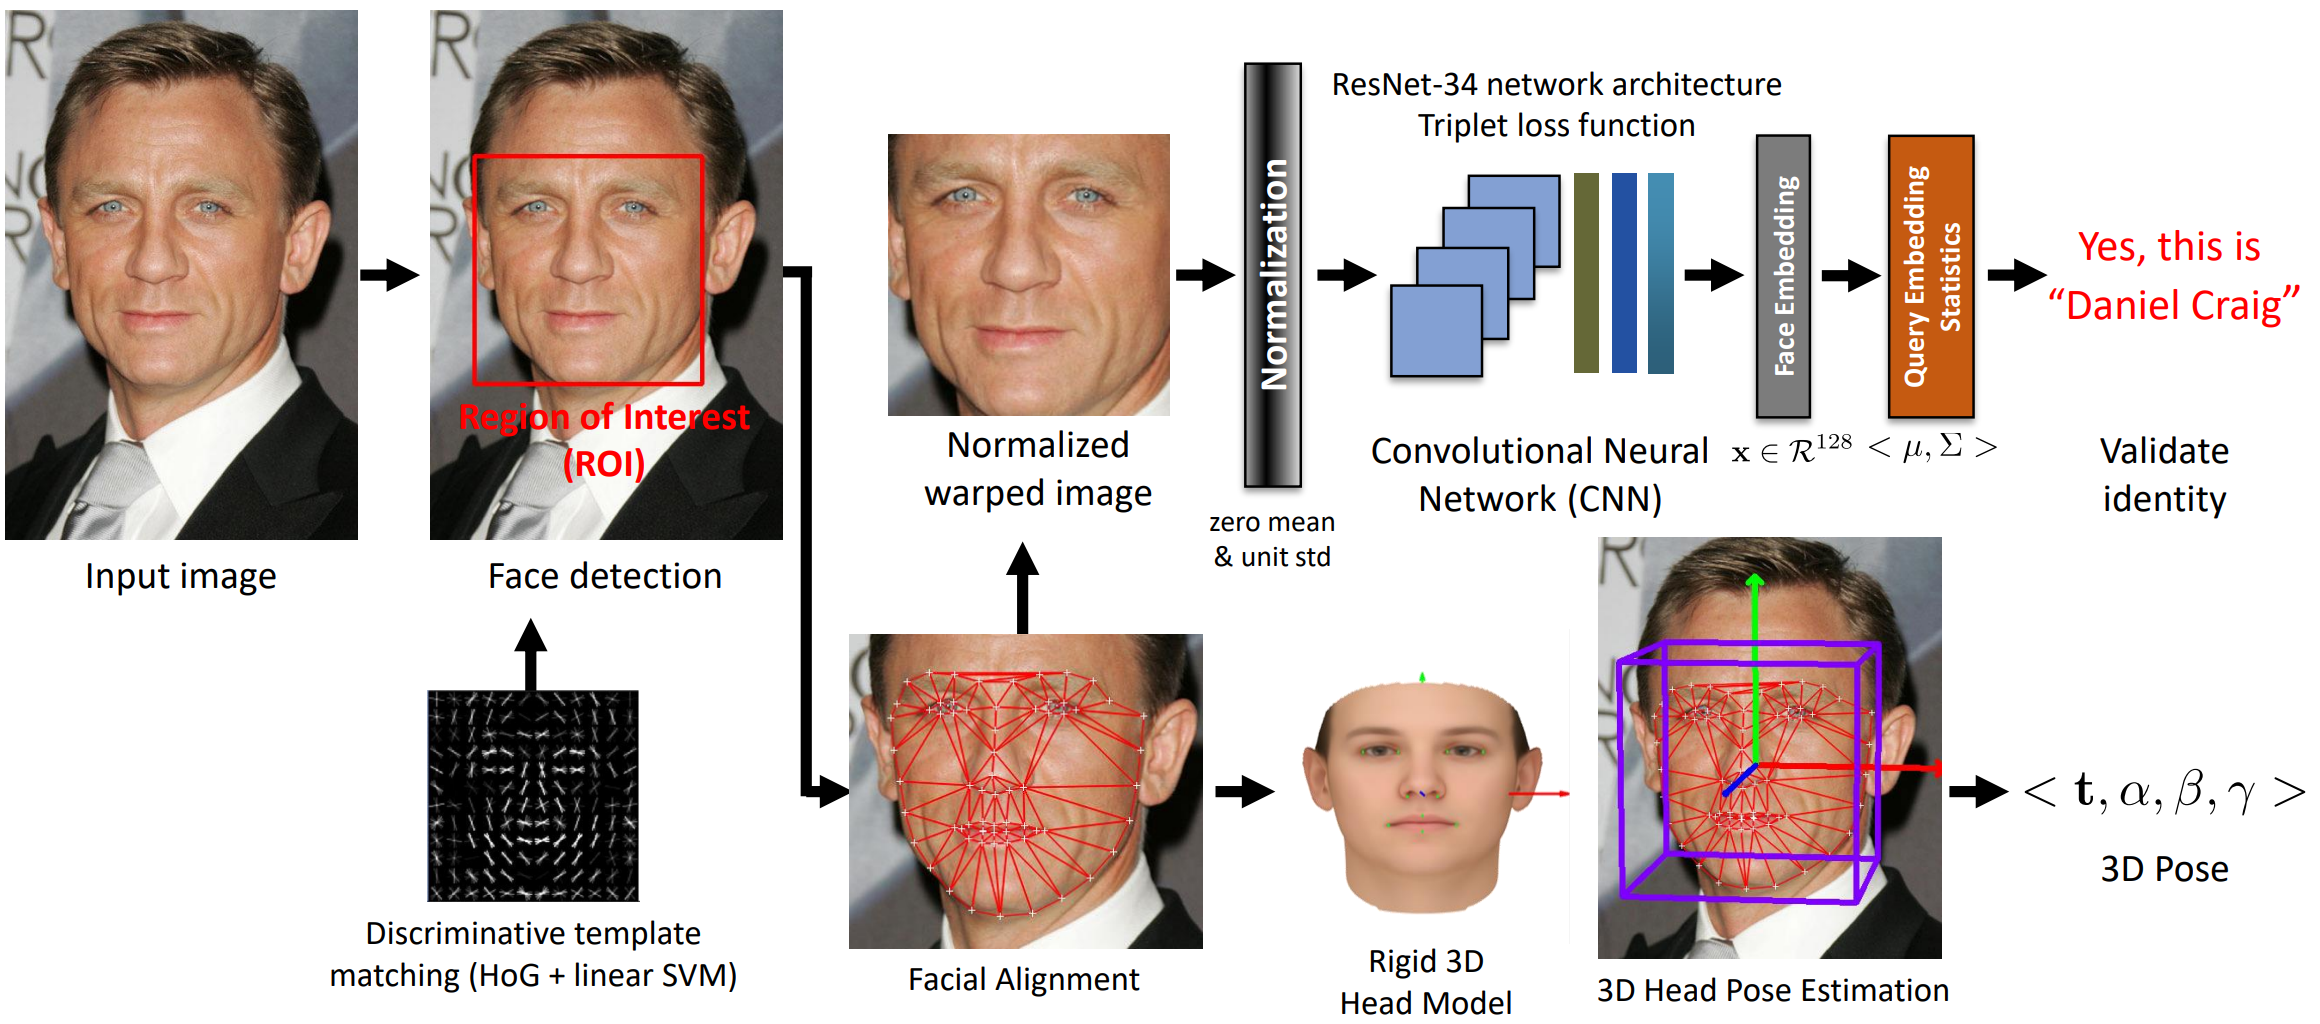
\includegraphics[scale=0.13]{trustid_arch.png}
    \caption[TrustID's Architecture.]{TrustID's Architecture. Image from the case study's paper~\autocite{fariaImagebasedFaceVerification2023}}
    \label{fig:trustid_arch}
  \end{figure}

\par Here we compare the following four models against the TrustID Resnet-34 based solution \reffig{fig:trustid_arch}, which comprises 29 layers, an average inference time of 7.28 seconds (computed by averaging the inference time on the entire dataset for all the benchmarks) and has been trained on the VGG Face and Facescrub ensemble dataset using triplet loss. Relevant specifications to assist the identification of a superior model are presented in \autoref{tab:models-table}. 

\begin{table}[H]
    \caption[Model's characteristics: ``\# Parameter'', ``\# Mult-Adds'', ``\# Layers'', ``Embedding'', ``Inference time (s)'', ``Loss'', and ``Dataset''.]{Model's characteristics. ``\# Parameter'' refers to the trainable parameters, ``\# Mult-Adds'' to the number of multiplication and addition operations, ``\# Layers'' denotes the quantity of convolutional and linear layers present in the model, ``Embedding'' signifies the dimensionality of the feature embedding produced by the model's output, ``Inference time (s)'' represents the average time taken for inference of all images from all the benchmark datasets, ``Loss'' is the loss function used to train the model, and ``Dataset'' are the training images.}
    \label{tab:models-table}
    \resizebox{\textwidth}{!}{%
    \begin{tabular}{l|c|c|c|c|c|c|c|}
    \cline{2-8}
                                        & \# Parameters & \multicolumn{1}{l|}{\# Mult-Adds (G)} & \# Layers & Embedding & Inference time (s) & Loss         & Dataset               \\ \hline
    \multicolumn{1}{|l|}{MobileFaceNet} & 1,200,512     & 56.62                                 & 17        & 512       & 2.79                & ArcFace      & MS1MV2                \\ \hline
    \multicolumn{1}{|l|}{iResnet-18}    & 24,025,600    & 668.15                                & 18        & 512       & 5.01                & ArcFace      & MS1MV2                \\ \hline
    \multicolumn{1}{|l|}{FaceNet}       & 28,907,599    & 152.21                                & 63        & 512       & 5.89                & Softmax      & CASIA-WebFace         \\ \hline
    \multicolumn{1}{|l|}{iResnet-SE-50} & 43,797,696    & 1610.00                               & 50        & 512       & 9.78                & ArcFace      & MS1MV2                \\ \hline
    \end{tabular}%
    }
\end{table}


\par This initial analysis suggests that MobileFaceNet has promising characteristics. It is the least complex model, therefore, is less prone to overfitting to new data and, most importantly, the amount of computational overhead created and inferece times are much inferior to the others at study. This is supported by the fewer number of convolutional and linear layers, trainable parameters and mult-adds. Albeit the similar depth to that of iResnet-18, MobileFaceNet has, approximately, $95\%$ fewer parameters, which is reflected on the number of total mult-adds. However, further investigation is required to determine whether the aforementioned characteristics might pose a bottleneck, potentially leading to a less robust solution with subpar performance. The ideal solution should strike a balance between adapting to new data and necessary computational costs.

\section{Benchmarking Results}
\subsection{Accuracy}

\par After performing 10-fold cross validation on all the benchmark datasets with the pretrained models, the mean accuracy is presented on the following table.

 

\begin{table}[H]
    \centering
    \caption{Model's face verification accuracy.}
    \label{tab:acc}
    \resizebox{\textwidth}{!}{%
    \begin{tabular}{|l|cc|cc|cc|cc|l}
    \cline{1-9}

  \multicolumn{1}{|c|}{\multirow{2}{*}{\diagbox{Models}{Datasets}}}      & \multicolumn{2}{c|}{\textit{Frontal group}}                           & \multicolumn{2}{c|}{\textit{Age group}}                               & \multicolumn{2}{c|}{\textit{Pose group}}                              & \multicolumn{2}{c|}{\textit{Hard group}}                              &  \\ \cline{2-9}
  \multicolumn{1}{|c|}{}                                                 & \multicolumn{1}{c|}{CFP-FF}           & LFW            & \multicolumn{1}{c|}{AgeDB30}          & CALFW          & \multicolumn{1}{c|}{CFP-FP}           & CPLFW          & \multicolumn{1}{c|}{VGGFace2}         & XQLFW          &  \\ \cline{1-9}
  \multicolumn{1}{|l|}{MobileFaceNet}                                    & \multicolumn{1}{c|}{0.9884}          & 0.9912          & \multicolumn{1}{c|}{0.9308}          & 0.9362          & \multicolumn{1}{c|}{0.8957}          & 0.8642          & \multicolumn{1}{c|}{0.9050}          & 0.5063          &  \\ \cline{1-9}
  \multicolumn{1}{|l|}{iResnet-18}                      & \multicolumn{1}{c|}{\textbf{0.9960}} & \textbf{0.9960} & \multicolumn{1}{c|}{\textbf{0.9728}} & \textbf{0.9555} & \multicolumn{1}{c|}{0.9414}          & 0.8943          & \multicolumn{1}{c|}{0.9198}          & 0.4943                           &  \\ \cline{1-9}
  \multicolumn{1}{|l|}{FaceNet}                         & \multicolumn{1}{c|}{0.8909}          & 0.9038          & \multicolumn{1}{c|}{0.7147}          & 0.7470          & \multicolumn{1}{c|}{0.7664}          & 0.6738          & \multicolumn{1}{c|}{0.7748}          & 0.5000                           &  \\ \cline{1-9}
  \multicolumn{1}{|l|}{TrustID}                         & \multicolumn{1}{c|}{0.8807}          & 0.9906          & \multicolumn{1}{c|}{0.7153}          & 0.7198          & \multicolumn{1}{c|}{0.7030}          & 0.6235          & \multicolumn{1}{c|}{0.7400}          & \textbf{0.6135}                  &  \\ \cline{1-9}
  \multicolumn{1}{|l|}{iResnet-SE-50}                   & \multicolumn{1}{c|}{0.9959}          & 0.9953          & \multicolumn{1}{c|}{0.9263}          & 0.9543          & \multicolumn{1}{c|}{\textbf{0.9457}} & \textbf{0.9047} & \multicolumn{1}{c|}{\textbf{0.9396}} & 0.5137                           &  \\ \cline{1-9}
  \end{tabular}%
  }
\end{table}

\par From \autoref{tab:acc}, we can see that iResnet-18 and iResnet-SE-50 have comparable performance. iResnet-18 achieves higher accuracy values on more datasets than any other model, however, iResnet-SE-50 performs better on the datasets where iResnet-18 does not, but only by a very small margin. Additionally, concerning the datasets where iResnet-SE-50 exhibited slightly lower performance, the accuracy scores are also very close. Specifically, between the two models, CFP-FF, LFW, CALFW, CFP-FP, CPLFW and VGGFace2 are all within a margin of error that can be attributed to non-deterministic behaviors in PyTorch, the libraries used, hardware, and/or CUDA. It is also important to note that, even though MobileFaceNet did not achieve the higher accuracy on any benchmark, the scores are the third best and considering its lightweight specifications highlighted in \autoref{tab:models-table}, the results are very promising and present a good example of accuracy and computational cost trade-off without compromising accuracy for student monitoring. Regarding the results from the extremely hard XQLFW, they are exceedingly low, approaching 0.5, for almost all the methods. This suggests that the model is producing outputs that resemble random guesses, which is exactly what occurs with FaceNet. The only exception is TrustID, which can be probably justified by the method of training. By resizing smaller training images to $150\times150$ there is a degradation in quality that leads to a model more prepared to handle these situations. 


\subsection{ROC Curves}
\par The previous table indicates that the three methods with superior performance, based exclusively on the accuracy at the best similarity threshold for each model and dataset, are the iResnet-SE-50, iResnet-18 and MobileFaceNet. To conduct a more thorough investigation allowing us to select the most appropriate model to be fine-tuned, the TAR values are computed for a range of FAR values and the ROC curves are generated. By inspecting how close the ROC curve is to the top left corner, the prime models can be determined since those are able to correctly identify more genuine matches while keeping the incorrect matches low. 

\begin{figure}[H]
    \centering
    \begin{adjustbox}{center, minipage=1.1\textwidth, margin=0cm -0.1cm 0cm -0.1cm}  % Adjust parameters as needed
        \begin{minipage}[c]{0.49\textwidth}
            \centering
            \includegraphics[width=0.8\textwidth]{pre_lfw_trained.eps}
            \caption{ROC Curves for the LFW benchmark from the Frontal group.}
            \label{fig:roc_lfw}
        \end{minipage}
        \hfill
        \begin{minipage}[c]{0.49\textwidth}
            \centering
            \includegraphics[width=0.8\textwidth]{pre_calfw_trained.eps}
            \caption{ROC Curves for the CALFW benchmark from the Age group.}
            \label{fig:roc_calfw}
        \end{minipage}
    \end{adjustbox}
    \vspace{-0.4cm}
  \end{figure}
\vspace{-1cm}
\begin{figure}[H]
  \begin{adjustbox}{center, minipage=1.1\textwidth, margin=0cm -0.1cm 0cm -0.1cm}  % Adjust parameters
      \begin{minipage}[c]{0.49\textwidth}
          \centering
          \includegraphics[width=0.8\textwidth]{pre_cplfw_trained.eps}
          \caption{ROC Curves for the CPLFW benchmark from the Pose group.}
          \label{fig:roc_cplfw}
      \end{minipage}
      \hfill
      \begin{minipage}[c]{0.49\textwidth}
          \centering
          \includegraphics[width=0.8\textwidth]{pre_xqlfw_trained.eps}
          \caption{ROC Curves for the XQLFW benchmark from the Hard group.}
          \label{fig:roc_xqlfw}
      \end{minipage}
  \end{adjustbox}
  \vspace{-0.4cm}
\end{figure}

\par The selected ROC curves support our initial assumptions. It is evident that, across the entire FAR range, the three top-performing models are iResnet-SE-50, iResnet-18, and MobileFacenet. With the exception of XQLFW in \reffig{fig:roc_xqlfw}, where all models, except TrustID, perform poorly and are close to random guessing, the remaining seven datasets consistently position these three models near the top-left corner. This pattern indicates strong model performance. In scenarios with low FAR values, where the model is less tolerant of incorrectly identifying impostors as matches, the number of correctly classified pairs (TAR) is higher. Please refer to \hyperref[appendix:roc_curves_appendix]{Appendix E} for the remaining from each benchmark group.

\begin{table}[H]
    \caption{TAR@FAR for all the models and benchmarks.}
    \label{tab:far_tar}
\begin{adjustbox}{center, margin=0cm -0.1cm -0.1cm -0.1cm}
    \resizebox{1.1\textwidth}{!}{
  \begin{tabular}{llccccccccccccllllll}
                                                  &                               & \multicolumn{1}{l}{}         & \multicolumn{1}{l}{}         & \multicolumn{1}{l}{}                                & \multicolumn{1}{l}{}         & \multicolumn{1}{l}{}         & \multicolumn{1}{l}{}         & \multicolumn{1}{l}{}         & \multicolumn{1}{l}{}         & \multicolumn{1}{l}{}         & \multicolumn{1}{l}{}         & \multicolumn{1}{l}{}         & \multicolumn{1}{l}{}         &  &  &  &  &  &  \\ \cline{3-14}
                                                  & \multicolumn{1}{l|}{}         & \multicolumn{3}{c|}{iResnet-SE-50}                                                                                & \multicolumn{2}{c|}{iResnet-18}                             & \multicolumn{3}{c|}{MobileFacenet}                                                         & \multicolumn{2}{c|}{FaceNet}                                & \multicolumn{2}{c|}{TrustID}                                &  &  &  &  &  &  \\ \cline{3-14}
                                                  & \multicolumn{1}{l|}{}         & \multicolumn{1}{c|}{$1e-4$}    & \multicolumn{1}{c|}{$1e-3$}    & \multicolumn{1}{c|}{1e-2}                           & \multicolumn{1}{c|}{$1e-3$}    & \multicolumn{1}{c|}{$1e-2$}    & \multicolumn{1}{c|}{$1e-4$}    & \multicolumn{1}{c|}{$1e-3$}    & \multicolumn{1}{c|}{$1e-2$}    & \multicolumn{1}{c|}{$1e-3$}    & \multicolumn{1}{c|}{$1e-2$}    & \multicolumn{1}{c|}{$1e-3$}    & \multicolumn{1}{c|}{$1e-2$}    &  &  &  &  &  &  \\ \cline{1-14}
  \multicolumn{1}{|c|}{}                          & \multicolumn{1}{l|}{CFP-FF}   & \multicolumn{1}{c|}{0.10000} & \multicolumn{1}{c|}{0.10000} & \multicolumn{1}{c|}{0.99771}                        & \multicolumn{1}{c|}{0.09886} & \multicolumn{1}{c|}{0.99743} & \multicolumn{1}{c|}{0.09057} & \multicolumn{1}{c|}{0.09600} & \multicolumn{1}{c|}{0.98657} & \multicolumn{1}{c|}{0.02886} & \multicolumn{1}{c|}{0.55257} & \multicolumn{1}{c|}{0.03314} & \multicolumn{1}{c|}{0.58114} &  &  &  &  &  &  \\ \cline{2-14}
  \multicolumn{1}{|c|}{\multirow{-2}{*}{Frontal}} & \multicolumn{1}{l|}{LFW}      & \multicolumn{1}{c|}{0.99067} & \multicolumn{1}{c|}{0.99333} & \multicolumn{1}{c|}{{0.99700}} & \multicolumn{1}{c|}{0.99100} & \multicolumn{1}{c|}{0.99600} & \multicolumn{1}{c|}{0.91467} & \multicolumn{1}{c|}{0.96933} & \multicolumn{1}{c|}{0.99167} & \multicolumn{1}{c|}{0.39900} & \multicolumn{1}{c|}{0.68800} & \multicolumn{1}{c|}{0.26967} & \multicolumn{1}{c|}{0.50567} &  &  &  &  &  &  \\ \cline{1-14}
  \multicolumn{1}{|l|}{}                          & \multicolumn{1}{l|}{AgeDB30}  & \multicolumn{1}{c|}{0.68267} & \multicolumn{1}{c|}{0.81700} & \multicolumn{1}{c|}{0.92600}                        & \multicolumn{1}{c|}{0.91533} & \multicolumn{1}{c|}{0.95300} & \multicolumn{1}{c|}{0.4950}  & \multicolumn{1}{c|}{0.59500} & \multicolumn{1}{c|}{0.80267} & \multicolumn{1}{c|}{0.02900} & \multicolumn{1}{c|}{0.14867} & \multicolumn{1}{c|}{0.03467} & \multicolumn{1}{c|}{0.11100} &  &  &  &  &  &  \\ \cline{2-14}
  \multicolumn{1}{|l|}{\multirow{-2}{*}{Age}}     & \multicolumn{1}{l|}{CALFW}    & \multicolumn{1}{c|}{0.86633} & \multicolumn{1}{c|}{0.88233} & \multicolumn{1}{c|}{0.91733}                        & \multicolumn{1}{c|}{0.90167} & \multicolumn{1}{c|}{0.91933} & \multicolumn{1}{c|}{0.68100} & \multicolumn{1}{c|}{0.75900} & \multicolumn{1}{c|}{0.87100} & \multicolumn{1}{c|}{0.07867} & \multicolumn{1}{c|}{0.26767} & \multicolumn{1}{c|}{0.05300} & \multicolumn{1}{c|}{0.18267} &  &  &  &  &  &  \\ \cline{1-14}
  \multicolumn{1}{|l|}{}                          & \multicolumn{1}{l|}{CFP-FP}   & \multicolumn{1}{c|}{0.07600} & \multicolumn{1}{c|}{0.07971} & \multicolumn{1}{c|}{0.87371}                        & \multicolumn{1}{c|}{0.07628} & \multicolumn{1}{c|}{0.87400} & \multicolumn{1}{c|}{0.04200} & \multicolumn{1}{c|}{0.05171} & \multicolumn{1}{c|}{0.69857} & \multicolumn{1}{c|}{0.00857} & \multicolumn{1}{c|}{0.22171} & \multicolumn{1}{c|}{0.00686} & \multicolumn{1}{c|}{0.12629} &  &  &  &  &  &  \\ \cline{2-14}
  \multicolumn{1}{|l|}{\multirow{-2}{*}{Pose}}    & \multicolumn{1}{l|}{CPLFW}    & \multicolumn{1}{c|}{0.37533} & \multicolumn{1}{c|}{0.58833} & \multicolumn{1}{c|}{0.7900}                         & \multicolumn{1}{c|}{0.66767} & \multicolumn{1}{c|}{0.75400} & \multicolumn{1}{c|}{0.06467} & \multicolumn{1}{c|}{0.17200} & \multicolumn{1}{c|}{0.64400} & \multicolumn{1}{c|}{0.00967} & \multicolumn{1}{c|}{0.12433} & \multicolumn{1}{c|}{0.01567} & \multicolumn{1}{c|}{0.07300} &  &  &  &  &  &  \\ \cline{1-14}
  \multicolumn{1}{|l|}{}                          & \multicolumn{1}{l|}{VGGFace2} & \multicolumn{1}{c|}{0.06000} & \multicolumn{1}{c|}{0.77280} & \multicolumn{1}{c|}{0.86280}                        & \multicolumn{1}{c|}{0.70320} & \multicolumn{1}{c|}{0.81840} & \multicolumn{1}{c|}{0.05240} & \multicolumn{1}{c|}{0.53880} & \multicolumn{1}{c|}{0.72160} & \multicolumn{1}{c|}{0.17000} & \multicolumn{1}{c|}{0.31720} & \multicolumn{1}{c|}{0.06640} & \multicolumn{1}{c|}{0.19400} &  &  &  &  &  &  \\ \cline{2-14}
  \multicolumn{1}{|l|}{\multirow{-2}{*}{Hard}}    & \multicolumn{1}{l|}{XQLFW}    & \multicolumn{1}{c|}{0.00001} & \multicolumn{1}{c|}{0.00033} & \multicolumn{1}{c|}{0.00800}                        & \multicolumn{1}{c|}{0.00033} & \multicolumn{1}{c|}{0.00433} & \multicolumn{1}{c|}{0.00001} & \multicolumn{1}{c|}{0.00100} & \multicolumn{1}{c|}{0.00433} & \multicolumn{1}{c|}{0.02000} & \multicolumn{1}{c|}{0.40433} & \multicolumn{1}{c|}{0.02167} & \multicolumn{1}{c|}{0.07867} &  &  &  &  &  &  \\ \cline{1-14}
  \end{tabular}%
    }
  \end{adjustbox}

\end{table}

The aforementioned three highest-achieving models distance themselves from FaceNet and TrustID on the ROC plots, although there is some overlap. As such, \autoref{tab:far_tar} allows us to analyze their performance at lower FAR values, where this overlap occurs. 
\par For a low FAR value of $1e-4$, the threshold is more firm and leaves less margin for identifying wrong matches as true identities, all models fail on more demanding datasets, but for less intricate ones, iResnet-SE-50 achieves suitable performance on LFW and CALFW, and MobileFaceNet on LFW. Reducing the strictness and increasing the FAR to $1e-3,$ leads to an improvement on the results, as expected. The iResnet models produce high TAR values on all datasets apart from the more challenging CFP variations and XQLFW datasets. MobileFacenet starts to improve but still performs poorly on the pose group, hard group, CFP pair and AgeDB30 dataset. Finally, at $1e-2$ is the threshold at which all models excel without compromising the security of the system, since increasing the FAR to $1e-1$ would lead to too much falsely matched pairs. iResnet-SE-50 and iResnet-18 have comparable performance with high scores on the same benchmarks and both failing XQLFW. MobileFaceNet approaches iResnet levels of capability aside from slightly lower scores on the age and pose groups and the XQLFW dataset.

\subsection{DET Curves}
To finalize the selection of the most appropriate model, the FRRs are calculated and plotted against the previous FAR values to obtain the DET curves. The intersection between the identity line that divides the graph and the DETs, i.e, the EER points can be extracted. These curves also allow to make a better distinction between models due to the more expansive logarithmic scale in which they are generated. In this case, contrary to the ROC curves, the better performing models are closer to the lower left corner, minimizing both the amount of impostors matched as true identities (FAR) and true identities classified as impostors (FRR).

\begin{figure}[H]
    \centering
    \begin{adjustbox}{center, minipage=1.1\textwidth, margin=0cm -0.1cm 0cm -0.1cm}  % Adjust parameters as needed
        \begin{minipage}[c]{0.49\textwidth}
            \centering
            \includegraphics[width=0.8\textwidth]{pre_lfw_dte_trained.eps}
            \caption{DET Curves for the LFW benchmark from the Frontal group.}
            \label{fig:dte_lfw}
        \end{minipage}
        \hfill
        \begin{minipage}[c]{0.49\textwidth}
            \centering
            \includegraphics[width=0.8\textwidth]{pre_calfw_dte_trained.eps}
            \caption{DET Curves for the CALFW benchmark from the Age group.}
            \label{fig:dte_calfw}
        \end{minipage}
    \end{adjustbox}
    \vspace{-0.4cm}
  \end{figure}
  
\begin{figure}[H]
\begin{adjustbox}{center, minipage=1.2\textwidth, margin=0cm -0.1cm 0cm -0.1cm}  % Adjust parameters
    \begin{minipage}[c]{0.49\textwidth}
        \centering
        \includegraphics[width=0.8\textwidth]{pre_cplfw_dte_trained.eps}
        \caption{DET Curves for the CPLFW benchmark from the Pose group.}
        \label{fig:dte_cplfw}
    \end{minipage}
    \hfill
    \begin{minipage}[c]{0.49\textwidth}
        \centering
        \includegraphics[width=0.8\textwidth]{pre_xqlfw_dte_trained.eps}
        \caption{DET Curves for the XQLFW benchmark from the Hard group.}
        \label{fig:dte_xqlfw}
    \end{minipage}
\end{adjustbox}
\vspace{-0.4cm}
\end{figure}

\vspace{0.9\baselineskip}
\begin{table}[H]
    \centering
    \caption{EER values for all the models and respective benchmarks.}
    \label{tab:eer_points}
    \resizebox{\textwidth}{!}{%
    \begin{tabular}{ll|cc|cc|cc|cc|}
    \cline{3-10}
                          &               & \multicolumn{2}{c|}{Frontal}                           & \multicolumn{2}{c|}{Age}                               & \multicolumn{2}{c|}{Pose}                              & \multicolumn{2}{c|}{Hard}                              \\ \cline{3-10} 
                          &               & \multicolumn{1}{c|}{CFP-FF}          & LFW             & \multicolumn{1}{c|}{AgeDB30}         & CALFW           & \multicolumn{1}{c|}{CFP-FP}          & CPLFW           & \multicolumn{1}{c|}{VGGFace2}        & XQLFW           \\ \cline{2-10} 
    \multicolumn{1}{l|}{} & MobileFaceNet & \multicolumn{1}{c|}{0.0126}          & 0.0090          & \multicolumn{1}{c|}{0.0723}          & 0.0727          & \multicolumn{1}{c|}{0.1069}          & 0.1463          & \multicolumn{1}{c|}{0.1020}          & 0.4849          \\ \cline{2-10} 
    \multicolumn{1}{l|}{} & iResnet-18    & \multicolumn{1}{c|}{0.0043}          & 0.0045          & \multicolumn{1}{c|}{\textbf{0.0297}} & 0.0617          & \multicolumn{1}{c|}{0.0609}          & 0.1220          & \multicolumn{1}{c|}{0.0882}          & 0.5094          \\ \cline{2-10} 
    \multicolumn{1}{l|}{} & FaceNet       & \multicolumn{1}{c|}{0.1111}          & 0.0957          & \multicolumn{1}{c|}{0.2900}          & 0.2517          & \multicolumn{1}{c|}{0.2326}          & 0.3270          & \multicolumn{1}{c|}{0.2276}          & -               \\ \cline{2-10} 
    \multicolumn{1}{l|}{} & TrustID       & \multicolumn{1}{c|}{0.1210}          & 0.1465          & \multicolumn{1}{c|}{0.2827}          & 0.2850          & \multicolumn{1}{c|}{0.2951}          & 0.3742          & \multicolumn{1}{c|}{0.2594}          & \textbf{0.3880} \\ \cline{2-10} 
    \multicolumn{1}{l|}{} & iResnet-SE-50 & \multicolumn{1}{c|}{\textbf{0.0040}} & \textbf{0.0043} & \multicolumn{1}{c|}{0.0723}          & \textbf{0.0577} & \multicolumn{1}{c|}{\textbf{0.0554}} & \textbf{0.1117} & \multicolumn{1}{c|}{\textbf{0.0708}} & 0.4854          \\ \cline{2-10} 
    \end{tabular}%
    }

\end{table}
\newpage
\par As a final analysis, the DET plots and the EER values support what has been previously discussed: iResnet-SE-50, iResnet-18 and MobileFaceNet are the best performing models. To no surprise, this group is always close to each other and close to the ideal corner of the DET graphs. Additionally, XQLFW reveals once again to be too much of a challenge. Regarding the EER scores, the results and conclusions are similar to the ones from \autoref{tab:acc}. iResnet-SE-50, the more complex model, has the lower scores, with iResnet-18 a close second and MobileFaceNet as the third. Please refer to \hyperref[appendix:det_curves_appendix]{Appendix F} for the remaining from each benchmark group

\section{Number of trainable parameters per unit of accuracy}

\par This metric is obtained by computing the division of the number of trainable parameters by the accuracy values, and it will serve as a complement to the metrics that evaluate resource's cost, i.e, the amount of mult-adds, inference time, and the number of trainable parameters and layers. Because the previous tests consecutively place iResnet-SE-50, iResnet-18 and MobileFaceNet as the more capable methods, they will be the ones studied in \autoref{tab:param_acc}. 

\begin{table}[H]
    \centering
    \caption{Number of trainable parameters per unit of accuracy for the three highest achieving models.}
    \label{tab:param_acc}
    \resizebox{\textwidth}{!}{%
    \begin{tabular}{|l|cc|cc|cc|cc|}
    \hline
    \multicolumn{1}{|c|}{\multirow{2}{*}{\diagbox{Models}{Datasets}}} & \multicolumn{2}{c|}{Frontal}           & \multicolumn{2}{c|}{Age}               & \multicolumn{2}{c|}{Pose}              & \multicolumn{2}{c|}{Hard}               \\ \cline{2-9} 
    \multicolumn{1}{|c|}{}                   & \multicolumn{1}{c|}{CFP-FF}  & LFW     & \multicolumn{1}{c|}{AgeDB30} & CALFW   & \multicolumn{1}{c|}{CFP-FP}  & CPLFW   & \multicolumn{1}{c|}{VGGFace2} & XQLFW   \\ \hline
    MobileFaceNet                            & \multicolumn{1}{c|}{\textbf{\num{1.216e6}}} & \textbf{\num{1.211e6}} & \multicolumn{1}{c|}{\textbf{\num{1.290e6}}} & \textbf{\num{1.282e6}} & \multicolumn{1}{c|}{\textbf{\num{1.340e6}}} & \textbf{\num{1.389e6}} & \multicolumn{1}{c|}{\textbf{\num{1.327e6}}}  & \textbf{\num{2.371e6}} \\ \hline
    iResnet-18                               & \multicolumn{1}{c|}{\num{2.412e7}} & \num{2.412e7} & \multicolumn{1}{c|}{\num{2.470e7}} & \num{2.514e7} & \multicolumn{1}{c|}{\num{2.552e7}} & \num{2.687e7} & \multicolumn{1}{c|}{\num{2.612e7}}  & \num{4.861e7} \\ \hline
    iResnet-SE-50                            & \multicolumn{1}{c|}{\num{4.398e7}} & \num{4.400e7} & \multicolumn{1}{c|}{\num{4.728e7}} & \num{4.590e7} & \multicolumn{1}{c|}{\num{4.631e7}} & \num{4.841e7} & \multicolumn{1}{c|}{\num{4.661e7}}  & \num{8.526e7} \\ \hline
    \end{tabular}%
    }
\end{table}

\par \autoref{tab:acc} emphasizes that the three methods attain comparable accuracy values, a crucial factor for model comparison with this metric. In this context, a lower NPUA value is preferred, as it indicates that a model can achieve the same accuracy while utilizing fewer trainable parameters. Finally, we can conclude that MobileFaceNet is the more computational cost-efficient, presenting NPUA scores lower than iResnet-18 and iResnet-SE-50 by, at least, an order of magnitude.


\subsection{Discussion}
\par At this stage, we are capable of assuring, based on the previous tests, that one objective is achieved and more adequate solutions to TrustID's facial verification framework were found. The three top performing methods proved their robustness to extreme variation in pose (CFP-FP and CPLFW), age (AgeDB30 and CALFW) or illumination (CFP-FF, VGGFace2). That being said, the benchmark concerning quality and image degradation (XQLFW) proved to be a major hurdle to most of the models aside from TrustID.

\par Considering the benchmarks' results, the much lower amount of trainable parameters, mult-adds, inference time and NPUA, MobileFaceNet is the best balance between performance and computational cost. As discussed in \autoref{sec:methodology_discussion}, due to the monitoring context, achieving perfect accuracy is not the main concern. This is due to the fact that, as the monitoring occurs over a time span it allows the system to perform more face verifications, compensating for lower accuracy values.
Furthermore, although it is true that MobileFacenet's accuracy is high in the pose group and VGGFace2, there is room for improvement in the TAR at low FAR values, hence the fine-tuning. The objective of further training the model first with QMUL-SurvFace is to try and improve its scores in both the hard group, specially XQLFW, and pose group benchmarks. On the other hand, DigiFace-1M enables the study of the impact of fully-synthetic ethically collected data on the scores throughout the benchmarks, with a special attention to the pose group benchmarks. 


\section{Training Details}
By leveraging Optuna's hyperparameter searching capabilities\footnote{\url{https://optuna.org/}}, we observe that the optimal combination is to train over batches of size 32 for 10 epochs with a $1e-4$ learning rate that decays according to a Cosine Annealing scheduler with warm up restarts. Additionally, because the model has Batch Normalization layers, they need to be explicitly set to evaluation mode during training. If this step is overlooked, the mean and variance used will be the ones from the batch and not the values achieved during the pre-training, leading to incorrect evaluation values. Following the original ArcFace work~\autocite{dengArcFaceAdditiveAngular}, the optimizer of choice is SGD with momentum $0.9$ and weight decay $5e-4$, scale $s=64$ and margin $m=0.5$. Manual early stopping is performed to ensure the most favorable achievable results, by evaluating on XQLFW and CPLFW during training and saving the model's training checkpoint with the highest performing accuracy. These validation datasets are selected accordingly to the areas where the models showed potential for improvement based on the benchmarks performed.

\section{Training Results}
% The following sections will gather the results from the several experiments that were performed in order to evaluate what solution is a better fit for the initial problem.
\subsection*{Fine-tuning all the layers}
\par The first approach is to update the whole network, since both QMUL-SurvFace and DigiFace-1M are large datasets with a high number of images and identities, there are less chances of quickly overfitting to the training data. \autoref{tab:acc_whole_qmul} and \autoref{tab:acc_whole_digiface} summarize the accuracy results for QMUL-SurvFace and DigiFace-1M, respectively.
\begin{table}[H]
    \centering
    \caption{MobileFaceNet accuracy scores before and after fine-tuning the whole network on QMUL-SurvFace with different ArcFace margins.}
    \label{tab:acc_whole_qmul}
    \resizebox{0.6\textwidth}{!}{%
    \begin{tabular}{|clc|c|c|c|}
    \hline
    \multicolumn{2}{|l|}{Benchmarks}                                                & Original                      & $m=0.5$                              & $m=0.4$                              & $m=0.3$                              \\ \hline
    \multicolumn{1}{|c|}{}                          & \multicolumn{1}{l|}{CFP-FF}   & {\color[HTML]{333333} 0.9884} & {\color[HTML]{333333} 0.7957 (\textcolor{red}{$\downarrow$})} & {\color[HTML]{333333} 0.7916 (\textcolor{red}{$\downarrow$})} & {\color[HTML]{333333} 0.7916 (\textcolor{red}{$\downarrow$})} \\ \cline{2-6} 
    \multicolumn{1}{|c|}{\multirow{-2}{*}{Frontal}} & \multicolumn{1}{l|}{LFW}      & {\color[HTML]{333333} 0.9912} & {\color[HTML]{333333} 0.7957 (\textcolor{red}{$\downarrow$})} & {\color[HTML]{333333} 0.7915 (\textcolor{red}{$\downarrow$})} & {\color[HTML]{333333} 0.7913 (\textcolor{red}{$\downarrow$})} \\ \hline
    \multicolumn{1}{|c|}{}                          & \multicolumn{1}{l|}{AgeDB30}  & {\color[HTML]{333333} 0.9308} & {\color[HTML]{333333} 0.6165 (\textcolor{red}{$\downarrow$})} & {\color[HTML]{333333} 0.6112 (\textcolor{red}{$\downarrow$})} & {\color[HTML]{333333} 0.6362 (\textcolor{red}{$\downarrow$})} \\ \cline{2-6} 
    \multicolumn{1}{|c|}{\multirow{-2}{*}{Age}}     & \multicolumn{1}{l|}{CALFW}    & {\color[HTML]{333333} 0.9362} & {\color[HTML]{333333} 0.6593 (\textcolor{red}{$\downarrow$})} & {\color[HTML]{333333} 0.6235 (\textcolor{red}{$\downarrow$})} & {\color[HTML]{333333} 0.6472 (\textcolor{red}{$\downarrow$})} \\ \hline
    \multicolumn{1}{|c|}{}                          & \multicolumn{1}{l|}{CFP-FP}   & {\color[HTML]{333333} 0.8957} & {\color[HTML]{333333} 0.6447 (\textcolor{red}{$\downarrow$})} & {\color[HTML]{333333} 0.6381 (\textcolor{red}{$\downarrow$})} & {\color[HTML]{333333} 0.6556 (\textcolor{red}{$\downarrow$})} \\ \cline{2-6} 
    \multicolumn{1}{|c|}{\multirow{-2}{*}{Pose}}    & \multicolumn{1}{l|}{CPLFW}    & {\color[HTML]{333333} 0.8642} & {\color[HTML]{333333} 0.6048 (\textcolor{red}{$\downarrow$})} & {\color[HTML]{333333} 0.5843 (\textcolor{red}{$\downarrow$})} & {\color[HTML]{333333} 0.5992 (\textcolor{red}{$\downarrow$})} \\ \hline
    \multicolumn{1}{|c|}{}                          & \multicolumn{1}{l|}{VGGFace2} & {\color[HTML]{333333} 0.9050} & {\color[HTML]{333333} 0.6516 (\textcolor{red}{$\downarrow$})} & {\color[HTML]{333333} 0.6188 (\textcolor{red}{$\downarrow$})} & {\color[HTML]{333333} 0.6314 (\textcolor{red}{$\downarrow$})} \\ \cline{2-6} 
    \multicolumn{1}{|c|}{\multirow{-2}{*}{Hard}}    & \multicolumn{1}{l|}{XQLFW}    & {\color[HTML]{333333} 0.5063} & {\color[HTML]{333333} 0.5325 (\textcolor{green}{$\uparrow$})}   & {\color[HTML]{333333} 0.5355 (\textcolor{green}{$\uparrow$})}   & {\color[HTML]{333333} 0.5215 (\textcolor{green}{$\uparrow$})}   \\ \hline
    \multicolumn{3}{|l|}{Stopping Epoch}                                                                            & 6                                  & 7                                  & 7                                  \\ \hline
    \end{tabular}%
    }
\end{table}

\par According to \autoref{tab:acc_whole_qmul}, fine-tuning with QMUL-SurvFace improves, as intended, the XQLFW benchmark performance by $5.17\%$. However, the verified increase is moderate and disadvantageous when the accuracy degradation verified on the remaining benchmarks is taken into account. Hence, in an effort to improve the results, the margin is reduced in order to generate a less penalizing training with a smaller distance between classes. The results from these settings are shown in \autoref{tab:acc_whole_qmul}, and when fine-tuned with QMUL-SurvFace, it occurs the same behavior as in $m=0.5$. The XQLFW results are also better than the original pre-trained model, increasing $5.77\%$ for $m=0.4$ and $3.00\%$ for $m=0.3$, while the other scores worsen. 
\begin{table}[H]
    \centering
    \caption{MobileFaceNet accuracy scores before and after fine-tuning the whole network on DigiFace-1M with different ArcFace margins.}
    \label{tab:acc_whole_digiface}
    \resizebox{0.6\textwidth}{!}{%
    \begin{tabular}{|clc|c|c|c|}
    \hline
    \multicolumn{2}{|l|}{Benchmarks}                                                & Original                      & $m=0.5$                              & $m=0.4$                              & $m=0.3$                              \\ \hline
    \multicolumn{1}{|c|}{}                          & \multicolumn{1}{l|}{CFP-FF}   & {\color[HTML]{333333} 0.9884} & {\color[HTML]{333333} 0.8011 (\textcolor{red}{$\downarrow$})} & {\color[HTML]{333333} 0.8231 (\textcolor{red}{$\downarrow$})} & {\color[HTML]{333333} 0.8157 (\textcolor{red}{$\downarrow$})} \\ \cline{2-6} 
    \multicolumn{1}{|c|}{\multirow{-2}{*}{Frontal}} & \multicolumn{1}{l|}{LFW}      & {\color[HTML]{333333} 0.9912} & {\color[HTML]{333333} 0.8011 (\textcolor{red}{$\downarrow$})} & {\color[HTML]{333333} 0.8231 (\textcolor{red}{$\downarrow$})} & {\color[HTML]{333333} 0.8157 (\textcolor{red}{$\downarrow$})} \\ \hline
    \multicolumn{1}{|c|}{}                          & \multicolumn{1}{l|}{AgeDB30}  & {\color[HTML]{333333} 0.9308} & {\color[HTML]{333333} 0.6732 (\textcolor{red}{$\downarrow$})} & {\color[HTML]{333333} 0.6733 (\textcolor{red}{$\downarrow$})} & {\color[HTML]{333333} 0.6723 (\textcolor{red}{$\downarrow$})} \\ \cline{2-6} 
    \multicolumn{1}{|c|}{\multirow{-2}{*}{Age}}     & \multicolumn{1}{l|}{CALFW}    & {\color[HTML]{333333} 0.9362} & {\color[HTML]{333333} 0.6755 (\textcolor{red}{$\downarrow$})} & {\color[HTML]{333333} 0.7010 (\textcolor{red}{$\downarrow$})} & {\color[HTML]{333333} 0.7010 (\textcolor{red}{$\downarrow$})} \\ \hline
    \multicolumn{1}{|c|}{}                          & \multicolumn{1}{l|}{CFP-FP}   & {\color[HTML]{333333} 0.8957} & {\color[HTML]{333333} 0.6191 (\textcolor{red}{$\downarrow$})} & {\color[HTML]{333333} 0.6483 (\textcolor{red}{$\downarrow$})} & {\color[HTML]{333333} 0.6609 (\textcolor{red}{$\downarrow$})} \\ \cline{2-6} 
    \multicolumn{1}{|c|}{\multirow{-2}{*}{Pose}}    & \multicolumn{1}{l|}{CPLFW}    & {\color[HTML]{333333} 0.8642} & {\color[HTML]{333333} 0.5945 (\textcolor{red}{$\downarrow$})} & {\color[HTML]{333333} 0.6078 (\textcolor{red}{$\downarrow$})} & {\color[HTML]{333333} 0.6170 (\textcolor{red}{$\downarrow$})} \\ \hline
    \multicolumn{1}{|c|}{}                          & \multicolumn{1}{l|}{VGGFace2} & {\color[HTML]{333333} 0.9050} & {\color[HTML]{333333} 0.6520 (\textcolor{red}{$\downarrow$})} & {\color[HTML]{333333} 0.6744 (\textcolor{red}{$\downarrow$})} & {\color[HTML]{333333} 0.6758 (\textcolor{red}{$\downarrow$})} \\ \cline{2-6} 
    \multicolumn{1}{|c|}{\multirow{-2}{*}{Hard}}    & \multicolumn{1}{l|}{XQLFW}    & {\color[HTML]{333333} 0.5063} & {\color[HTML]{333333} 0.4965 (\textcolor{red}{$\downarrow$})} & {\color[HTML]{333333} 0.5003 (\textcolor{red}{$\downarrow$})} & {\color[HTML]{333333} 0.4975 (\textcolor{red}{$\downarrow$})} \\ \hline
    \multicolumn{3}{|l|}{Stopping Epoch}                                                                            & 6                                  & 5                                  & 6                                  \\ \hline
    \end{tabular}%
    }
\end{table}

\par In the case of DigiFace-1M in \autoref{tab:acc_whole_digiface}, no discernible improvements were observed, and reducing the margin size did not yield any positive changes. Instead, the model appears to struggle in adapting to the dataset, resulting in adjustments to the weights that ultimately led to a deterioration in benchmark performance.  

\par When comparing directly with the paper's suggested margin ($m=0.5$), some conclusions can be drawn. The model fine-tuned with QMUL-SurvFace produces inferior results in the frontal and age groups for $m=0.4$ and $m=0.3$, the pose group is superior for both margins and the hard group is mixed, where VGGFace2 has lower performance for $m=0.4$ and $m=0.3$, and XQLFW improves for $m=0.4$ and not for $m=0.3$. On the other hand, when $m=0.4$ and $m=0.3$, the DigiFace-1M training saw a marginal improvement throughout the tests but still performs poorly. All in all, reducing the margin size does not have a meaningful impact on the accuracy results, aside from the XQLFW when tuned with QMUL-SurvFace.

\par To achieve a more profound understanding of how the model reacts to the data, \autoref{tab:tar_far_qmul} and \autoref{tab:tar_far_digiface} present the TAR at very low FAR.

\begin{table}[H]
    \centering
    \caption{TAR@FAR after fine-tuning the model with QMUL-SurvFace.}
    \label{tab:tar_far_qmul}
    \resizebox{\textwidth}{!}{%
    \begin{tabular}{cl|ccc|ccc|ccc|}
    \cline{3-11}
    \multicolumn{1}{l}{}                            &          & \multicolumn{3}{c|}{$m=0.5$}                                                                                                              & \multicolumn{3}{c|}{$m=0.4$}                                         & \multicolumn{3}{c|}{$m=0.3$}                                         \\ \hline
    \multicolumn{2}{|l|}{Benchmarks}                           & \multicolumn{1}{c|}{$1e-4$}                          & \multicolumn{1}{c|}{$1e-3$}                          & $1e-2$                          & \multicolumn{1}{c|}{$1e-4$}   & \multicolumn{1}{c|}{$1e-3$}   & $1e-2$   & \multicolumn{1}{c|}{$1e-4$}   & \multicolumn{1}{c|}{$1e-3$}   & $1e-2$   \\ \hline
    \multicolumn{1}{|c|}{}                          & CFP-FF   & \multicolumn{1}{c|}{{\color[HTML]{333333} 0.0140 (\textcolor{red}{$\downarrow$})}} & \multicolumn{1}{c|}{{\color[HTML]{333333} 0.0209 (\textcolor{red}{$\downarrow$})}} & {\color[HTML]{333333} 0.3486 (\textcolor{red}{$\downarrow$})} & \multicolumn{1}{c|}{0.0063 (\textcolor{red}{$\downarrow$})} & \multicolumn{1}{c|}{0.0154 (\textcolor{red}{$\downarrow$})} & 0.2940 (\textcolor{red}{$\downarrow$}) & \multicolumn{1}{c|}{0.0091 (\textcolor{red}{$\downarrow$})} & \multicolumn{1}{c|}{0.0169 (\textcolor{red}{$\downarrow$})} & 0.3097 (\textcolor{red}{$\downarrow$}) \\ \cline{2-11} 
    \multicolumn{1}{|c|}{\multirow{-2}{*}{Frontal}} & LFW      & \multicolumn{1}{c|}{{\color[HTML]{333333} 0.3099 (\textcolor{red}{$\downarrow$})}} & \multicolumn{1}{c|}{{\color[HTML]{333333} 0.3263 (\textcolor{red}{$\downarrow$})}} & {\color[HTML]{333333} 0.4760 (\textcolor{red}{$\downarrow$})} & \multicolumn{1}{c|}{0.1267 (\textcolor{red}{$\downarrow$})} & \multicolumn{1}{c|}{0.1680 (\textcolor{red}{$\downarrow$})} & 0.3940 (\textcolor{red}{$\downarrow$}) & \multicolumn{1}{c|}{0.1927 (\textcolor{red}{$\downarrow$})} & \multicolumn{1}{c|}{0.2310 (\textcolor{red}{$\downarrow$})} & 0.4697 (\textcolor{red}{$\downarrow$}) \\ \hline
    \multicolumn{1}{|c|}{}                          & AgeDB30  & \multicolumn{1}{c|}{{\color[HTML]{333333} 0.0050 (\textcolor{red}{$\downarrow$})}} & \multicolumn{1}{c|}{{\color[HTML]{333333} 0.0083 (\textcolor{red}{$\downarrow$})}} & {\color[HTML]{333333} 0.0867 (\textcolor{red}{$\downarrow$})} & \multicolumn{1}{c|}{0.0027 (\textcolor{red}{$\downarrow$})} & \multicolumn{1}{c|}{0.0053 (\textcolor{red}{$\downarrow$})} & 0.0730 (\textcolor{red}{$\downarrow$}) & \multicolumn{1}{c|}{0.0093 (\textcolor{red}{$\downarrow$})} & \multicolumn{1}{c|}{0.0240 (\textcolor{red}{$\downarrow$})} & 0.0860 (\textcolor{red}{$\downarrow$}) \\ \cline{2-11} 
    \multicolumn{1}{|c|}{\multirow{-2}{*}{Age}}     & CALFW    & \multicolumn{1}{c|}{{\color[HTML]{333333} 0.0313 (\textcolor{red}{$\downarrow$})}} & \multicolumn{1}{c|}{{\color[HTML]{333333} 0.8053 (\textcolor{green}{$\uparrow$})}} & {\color[HTML]{333333} 0.8053 (\textcolor{red}{$\downarrow$})} & \multicolumn{1}{c|}{0.0070 (\textcolor{red}{$\downarrow$})} & \multicolumn{1}{c|}{0.0323 (\textcolor{red}{$\downarrow$})} & 0.0827 (\textcolor{red}{$\downarrow$}) & \multicolumn{1}{c|}{0.0283 (\textcolor{red}{$\downarrow$})} & \multicolumn{1}{c|}{0.0340 (\textcolor{red}{$\downarrow$})} & 0.0920 (\textcolor{red}{$\downarrow$}) \\ \hline
    \multicolumn{1}{|c|}{}                          & CFP-FP   & \multicolumn{1}{c|}{{\color[HTML]{333333} 0.0006 (\textcolor{red}{$\downarrow$})}} & \multicolumn{1}{c|}{{\color[HTML]{333333} 0.9380 (\textcolor{green}{$\uparrow$})}} & {\color[HTML]{333333} 0.9380 (\textcolor{green}{$\uparrow$})} & \multicolumn{1}{c|}{0.0003 (\textcolor{red}{$\downarrow$})} & \multicolumn{1}{c|}{0.0003 (\textcolor{red}{$\downarrow$})} & 0.0666 (\textcolor{red}{$\downarrow$}) & \multicolumn{1}{c|}{0.0000 (\textcolor{red}{$\downarrow$})} & \multicolumn{1}{c|}{0.0003 (\textcolor{red}{$\downarrow$})} & 0.0626 (\textcolor{red}{$\downarrow$}) \\ \cline{2-11} 
    \multicolumn{1}{|c|}{\multirow{-2}{*}{Pose}}    & CPLFW    & \multicolumn{1}{c|}{{\color[HTML]{333333} 0.0060 (\textcolor{red}{$\downarrow$})}} & \multicolumn{1}{c|}{{\color[HTML]{333333} 0.9664 (\textcolor{green}{$\uparrow$})}} & {\color[HTML]{333333} 0.9664 (\textcolor{green}{$\uparrow$})} & \multicolumn{1}{c|}{0.0050 (\textcolor{red}{$\downarrow$})}  & \multicolumn{1}{c|}{0.0067 (\textcolor{red}{$\downarrow$})} & 0.0397 (\textcolor{red}{$\downarrow$}) & \multicolumn{1}{c|}{0.0073 (\textcolor{red}{$\downarrow$})} & \multicolumn{1}{c|}{0.0147 (\textcolor{red}{$\downarrow$})} & 0.0613 (\textcolor{red}{$\downarrow$}) \\ \hline
    \multicolumn{1}{|c|}{}                          & VGGFace2 & \multicolumn{1}{c|}{{\color[HTML]{333333} 0.0040 (\textcolor{red}{$\downarrow$})}} & \multicolumn{1}{c|}{{\color[HTML]{333333} 0.0536 (\textcolor{red}{$\downarrow$})}} & {\color[HTML]{333333} 0.1060 (\textcolor{red}{$\downarrow$})} & \multicolumn{1}{c|}{0.0036 (\textcolor{red}{$\downarrow$})} & \multicolumn{1}{c|}{0.0376 (\textcolor{red}{$\downarrow$})} & 0.0880 (\textcolor{red}{$\downarrow$}) & \multicolumn{1}{c|}{0.0040 (\textcolor{red}{$\downarrow$})} & \multicolumn{1}{c|}{0.0364 (\textcolor{red}{$\downarrow$})} & 0.1216 (\textcolor{red}{$\downarrow$}) \\ \cline{2-11} 
    \multicolumn{1}{|c|}{\multirow{-2}{*}{Hard}}    & XQLFW    & \multicolumn{1}{c|}{{\color[HTML]{333333} 0.0000 (\textcolor{red}{$\downarrow$})}} & \multicolumn{1}{c|}{{\color[HTML]{333333} 0.0023 (\textcolor{green}{$\uparrow$})}} & {\color[HTML]{333333} 0.0173 (\textcolor{green}{$\uparrow$})} & \multicolumn{1}{c|}{0.0000 (\textcolor{red}{$\downarrow$})} & \multicolumn{1}{c|}{0.0000 (\textcolor{red}{$\downarrow$})} & 0.0000 (\textcolor{red}{$\downarrow$}) & \multicolumn{1}{c|}{0.0000 (\textcolor{red}{$\downarrow$})} & \multicolumn{1}{c|}{0.0000 (\textcolor{red}{$\downarrow$})} & 0.0000 (\textcolor{red}{$\downarrow$}) \\ \hline
    \end{tabular}%
    }
\end{table}

The reduced margins $m=0.4$ and $m=0.3$ produce lower TAR scores at any FAR, including the very relevant frontal group. However, when $m=0.5$, there are some improvements. At $FAR=1e-3$ and $FAR=1e-2$, XQLFW increases slightly and the pose group suffers a significant improvement relative to its higher scores before fine-tuning ($44.7\%$ for CFP-FP at FAR $1e-3$ and $1e-2$, and $59.0\%$ for CPLFW at FAR equal to $1e-3$ and 1e-2).

\begin{table}[H]
    \centering
    \caption{TAR@FAR after fine-tuning the model with DigiFace-1M.}
    \label{tab:tar_far_digiface}
    \resizebox{\textwidth}{!}{%
    \begin{tabular}{cl|ccc|ccc|ccc|}
    \cline{3-11}
    \multicolumn{1}{l}{}                            &          & \multicolumn{3}{c|}{$m=0.5$}                                                                                                              & \multicolumn{3}{c|}{$m=0.4$}                                         & \multicolumn{3}{c|}{$m=0.3$}                                         \\ \hline
    \multicolumn{2}{|l|}{Benchmarks}                           & \multicolumn{1}{c|}{$1e-4$}                          & \multicolumn{1}{c|}{$1e-3$}                          & $1e-2$                          & \multicolumn{1}{c|}{$1e-4$}   & \multicolumn{1}{c|}{$1e-3$}   & $1e-2$   & \multicolumn{1}{c|}{$1e-4$}   & \multicolumn{1}{c|}{$1e-3$}   & $1e-2$   \\ \hline
    \multicolumn{1}{|c|}{}                          & CFP-FF   & \multicolumn{1}{c|}{{\color[HTML]{333333} 0.0020 (\textcolor{red}{$\downarrow$})}} & \multicolumn{1}{c|}{{\color[HTML]{333333} 0.0069 (\textcolor{red}{$\downarrow$})}} & {\color[HTML]{333333} 0.1906 (\textcolor{red}{$\downarrow$})} & \multicolumn{1}{c|}{0.0026 (\textcolor{red}{$\downarrow$})} & \multicolumn{1}{c|}{0.0111 (\textcolor{red}{$\downarrow$})} & 0.3580 (\textcolor{red}{$\downarrow$}) & \multicolumn{1}{c|}{0.0057 (\textcolor{red}{$\downarrow$})} & \multicolumn{1}{c|}{0.0109 (\textcolor{red}{$\downarrow$})} & 0.3606 (\textcolor{red}{$\downarrow$}) \\ \cline{2-11} 
    \multicolumn{1}{|c|}{\multirow{-2}{*}{Frontal}} & LFW      & \multicolumn{1}{c|}{{\color[HTML]{333333} 0.1633 (\textcolor{red}{$\downarrow$})}} & \multicolumn{1}{c|}{{\color[HTML]{333333} 0.2810 (\textcolor{red}{$\downarrow$})}} & {\color[HTML]{333333} 0.5520 (\textcolor{red}{$\downarrow$})} & \multicolumn{1}{c|}{0.2300 (\textcolor{red}{$\downarrow$})} & \multicolumn{1}{c|}{0.3403 (\textcolor{red}{$\downarrow$})} & 0.6310 (\textcolor{red}{$\downarrow$}) & \multicolumn{1}{c|}{0.2320 (\textcolor{red}{$\downarrow$})} & \multicolumn{1}{c|}{0.3743 (\textcolor{red}{$\downarrow$})} & 0.6113 (\textcolor{red}{$\downarrow$}) \\ \hline
    \multicolumn{1}{|c|}{}                          & AgeDB30  & \multicolumn{1}{c|}{{\color[HTML]{333333} 0.0013 (\textcolor{red}{$\downarrow$})}} & \multicolumn{1}{c|}{{\color[HTML]{333333} 0.0083 (\textcolor{red}{$\downarrow$})}} & {\color[HTML]{333333} 0.0530 (\textcolor{red}{$\downarrow$})} & \multicolumn{1}{c|}{0.0010 (\textcolor{red}{$\downarrow$})} & \multicolumn{1}{c|}{0.0153 (\textcolor{red}{$\downarrow$})} & 0.0747 (\textcolor{red}{$\downarrow$}) & \multicolumn{1}{c|}{0.0003 (\textcolor{red}{$\downarrow$})} & \multicolumn{1}{c|}{0.0250 (\textcolor{red}{$\downarrow$})} & 0.0790 (\textcolor{red}{$\downarrow$}) \\ \cline{2-11} 
    \multicolumn{1}{|c|}{\multirow{-2}{*}{Age}}     & CALFW    & \multicolumn{1}{c|}{{\color[HTML]{333333} 0.0017 (\textcolor{red}{$\downarrow$})}} & \multicolumn{1}{c|}{{\color[HTML]{333333} 0.0043 (\textcolor{red}{$\downarrow$})}} & {\color[HTML]{333333} 0.0780 (\textcolor{red}{$\downarrow$})} & \multicolumn{1}{c|}{0.0013 (\textcolor{red}{$\downarrow$})} & \multicolumn{1}{c|}{0.0300 (\textcolor{red}{$\downarrow$})} & 0.1207 (\textcolor{red}{$\downarrow$}) & \multicolumn{1}{c|}{0.0050 (\textcolor{red}{$\downarrow$})} & \multicolumn{1}{c|}{0.0170 (\textcolor{red}{$\downarrow$})} & 0.1223 (\textcolor{red}{$\downarrow$}) \\ \hline
    \multicolumn{1}{|c|}{}                          & CFP-FP   & \multicolumn{1}{c|}{{\color[HTML]{333333} 0.0000 (\textcolor{red}{$\downarrow$})}} & \multicolumn{1}{c|}{{\color[HTML]{333333} 0.0000 (\textcolor{red}{$\downarrow$})}} & {\color[HTML]{333333} 0.0149 (\textcolor{red}{$\downarrow$})} & \multicolumn{1}{c|}{0.0000 (\textcolor{red}{$\downarrow$})} & \multicolumn{1}{c|}{0.0000 (\textcolor{red}{$\downarrow$})} & 0.0194 (\textcolor{red}{$\downarrow$}) & \multicolumn{1}{c|}{0.0000 (\textcolor{red}{$\downarrow$})} & \multicolumn{1}{c|}{0.0003 (\textcolor{red}{$\downarrow$})} & 0.0226 (\textcolor{red}{$\downarrow$}) \\ \cline{2-11} 
    \multicolumn{1}{|c|}{\multirow{-2}{*}{Pose}}    & CPLFW    & \multicolumn{1}{c|}{{\color[HTML]{333333} 0.0013 (\textcolor{red}{$\downarrow$})}} & \multicolumn{1}{c|}{{\color[HTML]{333333} 0.0017 (\textcolor{red}{$\downarrow$})}} & {\color[HTML]{333333} 0.0190 (\textcolor{red}{$\downarrow$})} & \multicolumn{1}{c|}{0.0007 (\textcolor{red}{$\downarrow$})} & \multicolumn{1}{c|}{0.0016 (\textcolor{red}{$\downarrow$})} & 0.0263 (\textcolor{red}{$\downarrow$}) & \multicolumn{1}{c|}{0.0007 (\textcolor{red}{$\downarrow$})} & \multicolumn{1}{c|}{0.0033 (\textcolor{red}{$\downarrow$})} & 0.0287 (\textcolor{red}{$\downarrow$}) \\ \hline
    \multicolumn{1}{|c|}{}                          & VGGFace2 & \multicolumn{1}{c|}{{\color[HTML]{333333} 0.0000 (\textcolor{red}{$\downarrow$})}} & \multicolumn{1}{c|}{{\color[HTML]{333333} 0.0008 (\textcolor{red}{$\downarrow$})}} & {\color[HTML]{333333} 0.0220 (\textcolor{red}{$\downarrow$})} & \multicolumn{1}{c|}{0.0000 (\textcolor{red}{$\downarrow$})} & \multicolumn{1}{c|}{0.0020 (\textcolor{red}{$\downarrow$})} & 0.0404 (\textcolor{red}{$\downarrow$}) & \multicolumn{1}{c|}{0.0000 (\textcolor{red}{$\downarrow$})} & \multicolumn{1}{c|}{0.0028 (\textcolor{red}{$\downarrow$})} & 0.0440 (\textcolor{red}{$\downarrow$}) \\ \cline{2-11} 
    \multicolumn{1}{|c|}{\multirow{-2}{*}{Hard}}    & XQLFW    & \multicolumn{1}{c|}{{\color[HTML]{333333} 0.0000 (\textcolor{red}{$\downarrow$})}} & \multicolumn{1}{c|}{{\color[HTML]{333333} 0.0000 (\textcolor{red}{$\downarrow$})}} & {\color[HTML]{333333} 0.0083 (\textcolor{red}{$\downarrow$})} & \multicolumn{1}{c|}{0.0003 (\textcolor{green}{$\uparrow$})} & \multicolumn{1}{c|}{0.0013 (\textcolor{green}{$\uparrow$})} & 0.0087 (\textcolor{green}{$\uparrow$}) & \multicolumn{1}{c|}{0.0000 (\textcolor{red}{$\downarrow$})} & \multicolumn{1}{c|}{0.0010 (\textcolor{gray}{$-$})} & 0.0073 (\textcolor{green}{$\uparrow$}) \\ \hline
    \end{tabular}%
    }
\end{table}

\par Once again, the model trained with DigiFace-1M, does not perform and loses discriminative power at any margin and FAR value with the exception of a few outliers values that increase minimally, which can be seen as a mere fluctuation. 

\vspace{\baselineskip}

\par In the context of general CNN architectures, it is well-established that the initial layers are primarily responsible for learning fundamental features such as edges, basic shapes, and patterns that constitute objects or faces. Therefore, with the intention of improving the previous results, by preserving the weights associated with these earlier layers and avoiding introducing noise during further training, two other approaches are followed: 1) freeze the first 5 layers and 2) train only the 2 final layers. Additionally, based on the previous experiences, different ArcFace margins are also studied.
\vspace{3mm}

\subsection*{Fine-tuning with 5 initial frozen layers}
\autoref{tab:acc_5_qmul} and \autoref{tab:acc_5_digiface} present the accuracy scores after fine-tuning MobileFaceNet without updating the first five layers' weights. By freezing only 5 layers, the model still keeps its ability to learn more complex information associated with final stages of the network.

\begin{table}[H]
    \centering
    \caption{MobileFaceNet accuracy scores before and after fine-tuning the network, with the first five layers frozen, on QMUL-SurvFace with different ArcFace margins.}
    \label{tab:acc_5_qmul}
    \resizebox{0.6\textwidth}{!}{%
    \begin{tabular}{clcccc}
    \multicolumn{1}{l}{}                           &                               & \multicolumn{1}{l}{}          & \multicolumn{1}{l}{}             & \multicolumn{1}{l}{}             & \multicolumn{1}{l}{}             \\ \hline
    \multicolumn{2}{|l|}{Benchmarks}                                               & \multicolumn{1}{c|}{Original} & \multicolumn{1}{c|}{$m=0.5$}       & \multicolumn{1}{c|}{$m=0.4$}       & \multicolumn{1}{c|}{$m=0.3$}       \\ \hline
    \multicolumn{1}{|c|}{\multirow{2}{*}{Frontal}} & \multicolumn{1}{l|}{CFP-FF}   & \multicolumn{1}{c|}{0.9884}   & \multicolumn{1}{c|}{0.7821 (\textcolor{red}{$\downarrow$})} & \multicolumn{1}{c|}{0.8414 (\textcolor{red}{$\downarrow$})} & \multicolumn{1}{c|}{0.8155 (\textcolor{red}{$\downarrow$})} \\ \cline{2-6} 
    \multicolumn{1}{|c|}{}                         & \multicolumn{1}{l|}{LFW}      & \multicolumn{1}{c|}{0.9912}   & \multicolumn{1}{c|}{0.7820 (\textcolor{red}{$\downarrow$})} & \multicolumn{1}{c|}{0.8415 (\textcolor{red}{$\downarrow$})} & \multicolumn{1}{c|}{0.8156 (\textcolor{red}{$\downarrow$})} \\ \hline
    \multicolumn{1}{|c|}{\multirow{2}{*}{Age}}     & \multicolumn{1}{l|}{AgeDB30}  & \multicolumn{1}{c|}{0.9308}   & \multicolumn{1}{c|}{0.5985 (\textcolor{red}{$\downarrow$})} & \multicolumn{1}{c|}{0.6373 (\textcolor{red}{$\downarrow$})} & \multicolumn{1}{c|}{0.6382 (\textcolor{red}{$\downarrow$})} \\ \cline{2-6} 
    \multicolumn{1}{|c|}{}                         & \multicolumn{1}{l|}{CALFW}    & \multicolumn{1}{c|}{0.9362}   & \multicolumn{1}{c|}{0.6506 (\textcolor{red}{$\downarrow$})} & \multicolumn{1}{c|}{0.6962 (\textcolor{red}{$\downarrow$})} & \multicolumn{1}{c|}{0.6765 (\textcolor{red}{$\downarrow$})} \\ \hline
    \multicolumn{1}{|c|}{\multirow{2}{*}{Pose}}    & \multicolumn{1}{l|}{CFP-FP}   & \multicolumn{1}{c|}{0.8957}   & \multicolumn{1}{c|}{0.6477 (\textcolor{red}{$\downarrow$})} & \multicolumn{1}{c|}{0.6627 (\textcolor{red}{$\downarrow$})} & \multicolumn{1}{c|}{0.6499 (\textcolor{red}{$\downarrow$})} \\ \cline{2-6} 
    \multicolumn{1}{|c|}{}                         & \multicolumn{1}{l|}{CPLFW}    & \multicolumn{1}{c|}{0.8642}   & \multicolumn{1}{c|}{0.5943 (\textcolor{red}{$\downarrow$})} & \multicolumn{1}{c|}{0.6195 (\textcolor{red}{$\downarrow$})} & \multicolumn{1}{c|}{0.5872 (\textcolor{red}{$\downarrow$})} \\ \hline
    \multicolumn{1}{|c|}{\multirow{2}{*}{Hard}}    & \multicolumn{1}{l|}{VGGFace2} & \multicolumn{1}{c|}{0.9050}   & \multicolumn{1}{c|}{0.6442 (\textcolor{red}{$\downarrow$})} & \multicolumn{1}{c|}{0.6822 (\textcolor{red}{$\downarrow$})} & \multicolumn{1}{c|}{0.6610 (\textcolor{red}{$\downarrow$})} \\ \cline{2-6} 
    \multicolumn{1}{|c|}{}                         & \multicolumn{1}{l|}{XQLFW}    & \multicolumn{1}{c|}{0.5063}   & \multicolumn{1}{c|}{0.4925 (\textcolor{red}{$\downarrow$})} & \multicolumn{1}{c|}{0.5020 (\textcolor{red}{$\downarrow$})} & \multicolumn{1}{c|}{0.5127 (\textcolor{green}{$\uparrow$})}   \\ \hline
    \multicolumn{3}{|l|}{Stopping Epoch}                                                                           & \multicolumn{1}{c|}{8}           & \multicolumn{1}{c|}{5}           & \multicolumn{1}{c|}{6}           \\ \hline
    \end{tabular}%
    }
\end{table}

\begin{table}[H]
    \centering
    \caption{MobileFaceNet accuracy scores before and after fine-tuning the network, with the first five layers frozen, on DigiFace-1M with different ArcFace margins.}
    \label{tab:acc_5_digiface}
    \resizebox{0.6\textwidth}{!}{%
    \begin{tabular}{clcccc}
    \multicolumn{1}{l}{}                           &                               & \multicolumn{1}{l}{}          & \multicolumn{1}{l}{}             & \multicolumn{1}{l}{}             & \multicolumn{1}{l}{}             \\ \hline
    \multicolumn{2}{|l|}{Benchmarks}                                               & \multicolumn{1}{c|}{Original} & \multicolumn{1}{c|}{$m=0.5$}       & \multicolumn{1}{c|}{$m=0.4$}       & \multicolumn{1}{c|}{$m=0.3$}       \\ \hline
    \multicolumn{1}{|c|}{\multirow{2}{*}{Frontal}} & \multicolumn{1}{l|}{CFP-FF}   & \multicolumn{1}{c|}{0.9884}   & \multicolumn{1}{c|}{0.8840 (\textcolor{red}{$\downarrow$})} & \multicolumn{1}{c|}{0.8806 (\textcolor{red}{$\downarrow$})} & \multicolumn{1}{c|}{0.8788 (\textcolor{red}{$\downarrow$})} \\ \cline{2-6} 
    \multicolumn{1}{|c|}{}                         & \multicolumn{1}{l|}{LFW}      & \multicolumn{1}{c|}{0.9912}   & \multicolumn{1}{c|}{0.8840 (\textcolor{red}{$\downarrow$})} & \multicolumn{1}{c|}{0.8805 (\textcolor{red}{$\downarrow$})} & \multicolumn{1}{c|}{0.8789 (\textcolor{red}{$\downarrow$})} \\ \hline
    \multicolumn{1}{|c|}{\multirow{2}{*}{Age}}     & \multicolumn{1}{l|}{AgeDB30}  & \multicolumn{1}{c|}{0.9308}   & \multicolumn{1}{c|}{0.7265 (\textcolor{red}{$\downarrow$})} & \multicolumn{1}{c|}{0.7125 (\textcolor{red}{$\downarrow$})} & \multicolumn{1}{c|}{0.7303 (\textcolor{red}{$\downarrow$})} \\ \cline{2-6} 
    \multicolumn{1}{|c|}{}                         & \multicolumn{1}{l|}{CALFW}    & \multicolumn{1}{c|}{0.9362}   & \multicolumn{1}{c|}{0.7400 (\textcolor{red}{$\downarrow$})} & \multicolumn{1}{c|}{0.7478 (\textcolor{red}{$\downarrow$})} & \multicolumn{1}{c|}{0.7398 (\textcolor{red}{$\downarrow$})} \\ \hline
    \multicolumn{1}{|c|}{\multirow{2}{*}{Pose}}    & \multicolumn{1}{l|}{CFP-FP}   & \multicolumn{1}{c|}{0.8957}   & \multicolumn{1}{c|}{0.7219 (\textcolor{red}{$\downarrow$})} & \multicolumn{1}{c|}{0.7039 (\textcolor{red}{$\downarrow$})} & \multicolumn{1}{c|}{0.7223 (\textcolor{red}{$\downarrow$})} \\ \cline{2-6} 
    \multicolumn{1}{|c|}{}                         & \multicolumn{1}{l|}{CPLFW}    & \multicolumn{1}{c|}{0.8642}   & \multicolumn{1}{c|}{0.6423 (\textcolor{red}{$\downarrow$})} & \multicolumn{1}{c|}{0.6335 (\textcolor{red}{$\downarrow$})} & \multicolumn{1}{c|}{0.6435 (\textcolor{red}{$\downarrow$})} \\ \hline
    \multicolumn{1}{|c|}{\multirow{2}{*}{Hard}}    & \multicolumn{1}{l|}{VGGFace2} & \multicolumn{1}{c|}{0.9050}   & \multicolumn{1}{c|}{0.7220 (\textcolor{red}{$\downarrow$})} & \multicolumn{1}{c|}{0.7122 (\textcolor{red}{$\downarrow$})} & \multicolumn{1}{c|}{0.7080 (\textcolor{red}{$\downarrow$})} \\ \cline{2-6} 
    \multicolumn{1}{|c|}{}                         & \multicolumn{1}{l|}{XQLFW}    & \multicolumn{1}{c|}{0.5063}   & \multicolumn{1}{c|}{0.4997 (\textcolor{red}{$\downarrow$})} & \multicolumn{1}{c|}{0.4967 (\textcolor{red}{$\downarrow$})} & \multicolumn{1}{c|}{0.5033 (\textcolor{red}{$\downarrow$})} \\ \hline
    \multicolumn{3}{|l|}{Stopping Epoch}                                                                           & \multicolumn{1}{c|}{6}           & \multicolumn{1}{c|}{6}           & \multicolumn{1}{c|}{6}           \\ \hline
    \end{tabular}%
    }
\end{table}

As expected, the weights are less updated, hence the majority of the accuracy scores are higher than when training the whole network. Also, for QMUL-SurvFace (\autoref{tab:acc_5_qmul}), if $m=0.3$ there is even an improvement in the XQLFW benchmark. Finally, DigiFace-1M (\autoref{tab:acc_5_digiface}) at any $m$ value, shows no positive developments against the pre-trained model.

\begin{table}[H]
    \centering
    \caption{TAR@FAR after fine-tuning the model, with the first five layers frozen, on QMUL-SurvFace.}
    \label{tab:tar_far_5_qmul}
    \resizebox{\textwidth}{!}{%
    \begin{tabular}{cl|ccc|ccc|ccc|}
    \cline{3-11}
    \multicolumn{1}{l}{}                           &          & \multicolumn{3}{c|}{m=0.5}                                                        & \multicolumn{3}{c|}{m=0.4}                                                        & \multicolumn{3}{c|}{m=0.3}                                                        \\ \hline
    \multicolumn{2}{|l|}{Benchmarks}                          & \multicolumn{1}{c|}{1e-4}        & \multicolumn{1}{c|}{1e-3}        & 1e-2        & \multicolumn{1}{c|}{1e-4}        & \multicolumn{1}{c|}{1e-3}        & 1e-2        & \multicolumn{1}{c|}{1e-4}        & \multicolumn{1}{c|}{1e-3}        & 1e-2        \\ \hline
    \multicolumn{1}{|c|}{\multirow{2}{*}{Frontal}} & CFP-FF   & \multicolumn{1}{c|}{0.0117 (\textcolor{red}{$\downarrow$})} & \multicolumn{1}{c|}{0.0149 (\textcolor{red}{$\downarrow$})} & 0.2769 (\textcolor{red}{$\downarrow$}) & \multicolumn{1}{c|}{0.0174 (\textcolor{red}{$\downarrow$})} & \multicolumn{1}{c|}{0.0303 (\textcolor{red}{$\downarrow$})} & 0.4786 (\textcolor{red}{$\downarrow$}) & \multicolumn{1}{c|}{0.0163 (\textcolor{red}{$\downarrow$})} & \multicolumn{1}{c|}{0.0286 (\textcolor{red}{$\downarrow$})} & 0.3897 (\textcolor{red}{$\downarrow$}) \\ \cline{2-11} 
    \multicolumn{1}{|c|}{}                         & LFW      & \multicolumn{1}{c|}{0.2033 (\textcolor{red}{$\downarrow$})} & \multicolumn{1}{c|}{0.2277 (\textcolor{red}{$\downarrow$})} & 0.5047 (\textcolor{red}{$\downarrow$}) & \multicolumn{1}{c|}{0.2907 (\textcolor{red}{$\downarrow$})} & \multicolumn{1}{c|}{0.3473 (\textcolor{red}{$\downarrow$})} & 0.5870 (\textcolor{red}{$\downarrow$}) & \multicolumn{1}{c|}{0.2597 (\textcolor{red}{$\downarrow$})} & \multicolumn{1}{c|}{0.2743 (\textcolor{red}{$\downarrow$})} & 0.5533 (\textcolor{red}{$\downarrow$}) \\ \hline
    \multicolumn{1}{|c|}{\multirow{2}{*}{Age}}     & AgeDB30  & \multicolumn{1}{c|}{0.0137 (\textcolor{red}{$\downarrow$})} & \multicolumn{1}{c|}{0.0207 (\textcolor{red}{$\downarrow$})} & 0.0597 (\textcolor{red}{$\downarrow$}) & \multicolumn{1}{c|}{0.0087 (\textcolor{red}{$\downarrow$})} & \multicolumn{1}{c|}{0.0180 (\textcolor{red}{$\downarrow$})} & 0.0643 (\textcolor{red}{$\downarrow$}) & \multicolumn{1}{c|}{0.0063 (\textcolor{red}{$\downarrow$})} & \multicolumn{1}{c|}{0.0177 (\textcolor{red}{$\downarrow$})} & 0.0777 (\textcolor{red}{$\downarrow$}) \\ \cline{2-11} 
    \multicolumn{1}{|c|}{}                         & CALFW    & \multicolumn{1}{c|}{0.018 (\textcolor{red}{$\downarrow$})}  & \multicolumn{1}{c|}{0.0210 (\textcolor{red}{$\downarrow$})} & 0.0877 (\textcolor{red}{$\downarrow$}) & \multicolumn{1}{c|}{0.0667 (\textcolor{red}{$\downarrow$})} & \multicolumn{1}{c|}{0.0737 (\textcolor{red}{$\downarrow$})} & 0.1510 (\textcolor{red}{$\downarrow$}) & \multicolumn{1}{c|}{0.0267 (\textcolor{red}{$\downarrow$})} & \multicolumn{1}{c|}{0.0570 (\textcolor{red}{$\downarrow$})} & 0.1450 (\textcolor{red}{$\downarrow$}) \\ \hline
    \multicolumn{1}{|c|}{\multirow{2}{*}{Pose}}    & CFP-FP   & \multicolumn{1}{c|}{0.0000 (\textcolor{red}{$\downarrow$})} & \multicolumn{1}{c|}{0.0009 (\textcolor{red}{$\downarrow$})} & 0.0617 (\textcolor{red}{$\downarrow$}) & \multicolumn{1}{c|}{0.0011 (\textcolor{red}{$\downarrow$})} & \multicolumn{1}{c|}{0.0029 (\textcolor{red}{$\downarrow$})} & 0.0871 (\textcolor{red}{$\downarrow$}) & \multicolumn{1}{c|}{0.0009 (\textcolor{red}{$\downarrow$})} & \multicolumn{1}{c|}{0.0020 (\textcolor{red}{$\downarrow$})} & 0.0694 (\textcolor{red}{$\downarrow$}) \\ \cline{2-11} 
    \multicolumn{1}{|c|}{}                         & CPLFW    & \multicolumn{1}{c|}{0.0070 (\textcolor{red}{$\downarrow$})} & \multicolumn{1}{c|}{0.0170 (\textcolor{red}{$\downarrow$})} & 0.0570 (\textcolor{red}{$\downarrow$}) & \multicolumn{1}{c|}{0.0100 (\textcolor{red}{$\downarrow$})} & \multicolumn{1}{c|}{0.0183 (\textcolor{red}{$\downarrow$})} & 0.0870 (\textcolor{red}{$\downarrow$}) & \multicolumn{1}{c|}{0.0093 (\textcolor{red}{$\downarrow$})} & \multicolumn{1}{c|}{0.0187 (\textcolor{red}{$\downarrow$})} & 0.0633 (\textcolor{red}{$\downarrow$}) \\ \hline
    \multicolumn{1}{|c|}{\multirow{2}{*}{Hard}}    & VGGFace2 & \multicolumn{1}{c|}{0.0032 (\textcolor{red}{$\downarrow$})} & \multicolumn{1}{c|}{0.0352 (\textcolor{red}{$\downarrow$})} & 0.1112 (\textcolor{red}{$\downarrow$}) & \multicolumn{1}{c|}{0.0056 (\textcolor{red}{$\downarrow$})} & \multicolumn{1}{c|}{0.0712 (\textcolor{red}{$\downarrow$})} & 0.1516 (\textcolor{red}{$\downarrow$}) & \multicolumn{1}{c|}{0.0040 (\textcolor{red}{$\downarrow$})} & \multicolumn{1}{c|}{0.0528 (\textcolor{red}{$\downarrow$})} & 0.1304 (\textcolor{red}{$\downarrow$}) \\ \cline{2-11} 
    \multicolumn{1}{|c|}{}                         & XQLFW    & \multicolumn{1}{c|}{0.0000 (\textcolor{red}{$\downarrow$})} & \multicolumn{1}{c|}{0.0000 (\textcolor{red}{$\downarrow$})} & 0.0000 (\textcolor{red}{$\downarrow$}) & \multicolumn{1}{c|}{0.0000 (\textcolor{red}{$\downarrow$})} & \multicolumn{1}{c|}{0.0000 (\textcolor{red}{$\downarrow$})} & 0.0040 (\textcolor{red}{$\downarrow$}) & \multicolumn{1}{c|}{0.0000 (\textcolor{red}{$\downarrow$})} & \multicolumn{1}{c|}{0.0003 (\textcolor{red}{$\downarrow$})} & 0.0037(\textcolor{red}{$\downarrow$})  \\ \hline
    \end{tabular}%
    }
\end{table}

\begin{table}[H]
    \centering
    \caption{TAR@FAR after fine-tuning the model, with the first five layers frozen, on DigiFace-1M.}
    \label{tab:tar_far_5_digiface}
    \resizebox{\textwidth}{!}{%
    \begin{tabular}{cl|ccc|ccc|ccc|}
    \cline{3-11}
    \multicolumn{1}{l}{}                           &          & \multicolumn{3}{c|}{m=0.5}                                                        & \multicolumn{3}{c|}{m=0.4}                                                        & \multicolumn{3}{c|}{m=0.3}                                                        \\ \hline
    \multicolumn{2}{|l|}{Benchmarks}                          & \multicolumn{1}{c|}{1e-4}        & \multicolumn{1}{c|}{1e-3}        & 1e-2        & \multicolumn{1}{c|}{1e-4}        & \multicolumn{1}{c|}{1e-3}        & 1e-2        & \multicolumn{1}{c|}{1e-4}        & \multicolumn{1}{c|}{1e-3}        & 1e-2        \\ \hline
    \multicolumn{1}{|c|}{\multirow{2}{*}{Frontal}} & CFP-FF   & \multicolumn{1}{c|}{0.0189 (\textcolor{red}{$\downarrow$})} & \multicolumn{1}{c|}{0.0354 (\textcolor{red}{$\downarrow$})} & 0.5574 (\textcolor{red}{$\downarrow$}) & \multicolumn{1}{c|}{0.0183 (\textcolor{red}{$\downarrow$})} & \multicolumn{1}{c|}{0.0303 (\textcolor{red}{$\downarrow$})} & 0.5200 (\textcolor{red}{$\downarrow$}) & \multicolumn{1}{c|}{0.0294 (\textcolor{red}{$\downarrow$})} & \multicolumn{1}{c|}{0.0346 (\textcolor{red}{$\downarrow$})} & 0.5539 (\textcolor{red}{$\downarrow$}) \\ \cline{2-11} 
    \multicolumn{1}{|c|}{}                         & LFW      & \multicolumn{1}{c|}{0.3207 (\textcolor{red}{$\downarrow$})} & \multicolumn{1}{c|}{0.5577 (\textcolor{red}{$\downarrow$})} & 0.7440 (\textcolor{red}{$\downarrow$}) & \multicolumn{1}{c|}{0.2677 (\textcolor{red}{$\downarrow$})} & \multicolumn{1}{c|}{0.5180 (\textcolor{red}{$\downarrow$})} & 0.7360 (\textcolor{red}{$\downarrow$}) & \multicolumn{1}{c|}{0.4420 (\textcolor{red}{$\downarrow$})} & \multicolumn{1}{c|}{0.5980 (\textcolor{red}{$\downarrow$})} & 0.7497 (\textcolor{red}{$\downarrow$}) \\ \hline
    \multicolumn{1}{|c|}{\multirow{2}{*}{Age}}     & AgeDB30  & \multicolumn{1}{c|}{0.0083 (\textcolor{red}{$\downarrow$})} & \multicolumn{1}{c|}{0.0363 (\textcolor{red}{$\downarrow$})} & 0.1450 (\textcolor{red}{$\downarrow$}) & \multicolumn{1}{c|}{0.0027 (\textcolor{red}{$\downarrow$})} & \multicolumn{1}{c|}{0.0203 (\textcolor{red}{$\downarrow$})} & 0.1407 (\textcolor{red}{$\downarrow$}) & \multicolumn{1}{c|}{0.0047 (\textcolor{red}{$\downarrow$})} & \multicolumn{1}{c|}{0.0253 (\textcolor{red}{$\downarrow$})} & 0.1353 (\textcolor{red}{$\downarrow$}) \\ \cline{2-11} 
    \multicolumn{1}{|c|}{}                         & CALFW    & \multicolumn{1}{c|}{0.0407 (\textcolor{red}{$\downarrow$})} & \multicolumn{1}{c|}{0.0813 (\textcolor{red}{$\downarrow$})} & 0.2690 (\textcolor{red}{$\downarrow$}) & \multicolumn{1}{c|}{0.0100 (\textcolor{red}{$\downarrow$})} & \multicolumn{1}{c|}{0.0593 (\textcolor{red}{$\downarrow$})} & 0.2423 (\textcolor{red}{$\downarrow$}) & \multicolumn{1}{c|}{0.0150 (\textcolor{red}{$\downarrow$})} & \multicolumn{1}{c|}{0.0393 (\textcolor{red}{$\downarrow$})} & 0.2590 (\textcolor{red}{$\downarrow$}) \\ \hline
    \multicolumn{1}{|c|}{\multirow{2}{*}{Pose}}    & CFP-FP   & \multicolumn{1}{c|}{0.0006 (\textcolor{red}{$\downarrow$})} & \multicolumn{1}{c|}{0.0026 (\textcolor{red}{$\downarrow$})} & 0.1231 (\textcolor{red}{$\downarrow$}) & \multicolumn{1}{c|}{0.0003 (\textcolor{red}{$\downarrow$})} & \multicolumn{1}{c|}{0.0029 (\textcolor{red}{$\downarrow$})} & 0.0880 (\textcolor{red}{$\downarrow$}) & \multicolumn{1}{c|}{0.0003 (\textcolor{red}{$\downarrow$})} & \multicolumn{1}{c|}{0.0017 (\textcolor{red}{$\downarrow$})} & 0.1106 (\textcolor{red}{$\downarrow$}) \\ \cline{2-11} 
    \multicolumn{1}{|c|}{}                         & CPLFW    & \multicolumn{1}{c|}{0.0003 (\textcolor{red}{$\downarrow$})} & \multicolumn{1}{c|}{0.0017 (\textcolor{red}{$\downarrow$})} & 0.0383 (\textcolor{red}{$\downarrow$}) & \multicolumn{1}{c|}{0.0007 (\textcolor{red}{$\downarrow$})} & \multicolumn{1}{c|}{0.0023 (\textcolor{red}{$\downarrow$})} & 0.0247 (\textcolor{red}{$\downarrow$}) & \multicolumn{1}{c|}{0.0003 (\textcolor{red}{$\downarrow$})} & \multicolumn{1}{c|}{0.0017 (\textcolor{red}{$\downarrow$})} & 0.0407 (\textcolor{red}{$\downarrow$}) \\ \hline
    \multicolumn{1}{|c|}{\multirow{2}{*}{Hard}}    & VGGFace2 & \multicolumn{1}{c|}{0.0000 (\textcolor{red}{$\downarrow$})} & \multicolumn{1}{c|}{0.0176 (\textcolor{red}{$\downarrow$})} & 0.1732 (\textcolor{red}{$\downarrow$}) & \multicolumn{1}{c|}{0.0000 (\textcolor{red}{$\downarrow$})} & \multicolumn{1}{c|}{0.0056 (\textcolor{red}{$\downarrow$})} & 0.1392 (\textcolor{red}{$\downarrow$}) & \multicolumn{1}{c|}{0.0000 (\textcolor{red}{$\downarrow$})} & \multicolumn{1}{c|}{0.0040 (\textcolor{red}{$\downarrow$})} & 0.1468 (\textcolor{red}{$\downarrow$}) \\ \cline{2-11} 
    \multicolumn{1}{|c|}{}                         & XQLFW    & \multicolumn{1}{c|}{0.0000 (\textcolor{red}{$\downarrow$})} & \multicolumn{1}{c|}{0.0010 (\textcolor{gray}{$-$})} & 0.0100 (\textcolor{green}{$\uparrow$})   & \multicolumn{1}{c|}{0.0003 (\textcolor{green}{$\uparrow$})}   & \multicolumn{1}{c|}{0.0007 (\textcolor{red}{$\downarrow$})} & 0.0067 (\textcolor{green}{$\uparrow$})   & \multicolumn{1}{c|}{0.0000 (\textcolor{red}{$\downarrow$})} & \multicolumn{1}{c|}{0.0010 (\textcolor{gray}{$-$})} & 0.0093 (\textcolor{green}{$\uparrow$})   \\ \hline
    \end{tabular}%
    }
\end{table}

\par Finally, \autoref{tab:tar_far_5_qmul} and \autoref{tab:tar_far_5_digiface} highlight that training with less layers does not improve the performance at any FAR or margin. Moreover, the previous enhancements verified when the complete model is trained with QMUL-SurvFace with $m=0.5$, and $FAR=1e-3$ and $FAR=1e-2$ are lost with this configuration.


\subsection*{Fine-tuning the last 2 layers}

To finalize, we conducted additional tests by training only the last two layers (one convolutional and linear). This allows us to investigate in which direction the model evolves in terms of results when even less stages are trained.

\begin{table}[H]
    \centering
    \caption{MobileFaceNet accuracy scores before and after fine-tuning the network, with all the layers frozen aside the last two, on QMUL-SurvFace with different ArcFace margins.}
    \label{tab:acc_final_qmul}
    \resizebox{0.6\textwidth}{!}{%
    \begin{tabular}{|clc|c|c|c|}
    \hline
    \multicolumn{2}{|l|}{Benchmarks}                                               & Original & $m=0.5$       & $m=0.4$       & $m=0.3$       \\ \hline
    \multicolumn{1}{|c|}{\multirow{2}{*}{Frontal}} & \multicolumn{1}{l|}{CFP-FF}   & 0.9884   & 0.8751 (\textcolor{red}{$\downarrow$}) & 0.8821 (\textcolor{red}{$\downarrow$}) & 0.8786 (\textcolor{red}{$\downarrow$}) \\ \cline{2-6} 
    \multicolumn{1}{|c|}{}                         & \multicolumn{1}{l|}{LFW}      & 0.9912   & 0.8751 (\textcolor{red}{$\downarrow$}) & 0.8821 (\textcolor{red}{$\downarrow$}) & 0.8785 (\textcolor{red}{$\downarrow$}) \\ \hline
    \multicolumn{1}{|c|}{\multirow{2}{*}{Age}}     & \multicolumn{1}{l|}{AgeDB30}  & 0.9308   & 0.7097 (\textcolor{red}{$\downarrow$}) & 0.7220 (\textcolor{red}{$\downarrow$}) & 0.7080 (\textcolor{red}{$\downarrow$}) \\ \cline{2-6} 
    \multicolumn{1}{|c|}{}                         & \multicolumn{1}{l|}{CALFW}    & 0.9362   & 0.7762 (\textcolor{red}{$\downarrow$}) & 0.7833 (\textcolor{red}{$\downarrow$}) & 0.7752 (\textcolor{red}{$\downarrow$}) \\ \hline
    \multicolumn{1}{|c|}{\multirow{2}{*}{Pose}}    & \multicolumn{1}{l|}{CFP-FP}   & 0.8957   & 0.6729 (\textcolor{red}{$\downarrow$}) & 0.6714 (\textcolor{red}{$\downarrow$}) & 0.6719 (\textcolor{red}{$\downarrow$}) \\ \cline{2-6} 
    \multicolumn{1}{|c|}{}                         & \multicolumn{1}{l|}{CPLFW}    & 0.8642   & 0.6585 (\textcolor{red}{$\downarrow$}) & 0.6635 (\textcolor{red}{$\downarrow$}) & 0.6635 (\textcolor{red}{$\downarrow$}) \\ \hline
    \multicolumn{1}{|c|}{\multirow{2}{*}{Hard}}    & \multicolumn{1}{l|}{VGGFace2} & 0.9050   & 0.6992 (\textcolor{red}{$\downarrow$}) & 0.7014 (\textcolor{red}{$\downarrow$}) & 0.7006 (\textcolor{red}{$\downarrow$}) \\ \cline{2-6} 
    \multicolumn{1}{|c|}{}                         & \multicolumn{1}{l|}{XQLFW}    & 0.5063   & 0.4975 (\textcolor{red}{$\downarrow$}) & 0.4993 (\textcolor{red}{$\downarrow$}) & 0.5010 (\textcolor{red}{$\downarrow$}) \\ \hline
    \multicolumn{3}{|l|}{Stopping Epoch}                                                      & 6           & 3           & 6           \\ \hline
    \end{tabular}%
    }
\end{table}

\begin{table}[H]
    \centering
    \caption{MobileFaceNet accuracy scores before and after fine-tuning the network, with all the layers frozen aside the last two, on DigiFace-1M with different ArcFace margins.}
    \label{tab:acc_final_digiface}
    \resizebox{0.6\textwidth}{!}{%
    \begin{tabular}{|clc|c|c|c|}
    \hline
    \multicolumn{2}{|l|}{Benchmarks}                                               & Original & $m=0.5$       & $m=0.4$       & $m=0.3$       \\ \hline
    \multicolumn{1}{|c|}{\multirow{2}{*}{Frontal}} & \multicolumn{1}{l|}{CFP-FF}   & 0.9884   & 0.9568 (\textcolor{red}{$\downarrow$}) & 0.9630 (\textcolor{red}{$\downarrow$}) & 0.9574 (\textcolor{red}{$\downarrow$}) \\ \cline{2-6} 
    \multicolumn{1}{|c|}{}                         & \multicolumn{1}{l|}{LFW}      & 0.9912   & 0.9569 (\textcolor{red}{$\downarrow$}) & 0.9629 (\textcolor{red}{$\downarrow$}) & 0.9574 (\textcolor{red}{$\downarrow$}) \\ \hline
    \multicolumn{1}{|c|}{\multirow{2}{*}{Age}}     & \multicolumn{1}{l|}{AgeDB30}  & 0.9308   & 0.8420 (\textcolor{red}{$\downarrow$}) & 0.8533 (\textcolor{red}{$\downarrow$}) & 0.8403 (\textcolor{red}{$\downarrow$}) \\ \cline{2-6} 
    \multicolumn{1}{|c|}{}                         & \multicolumn{1}{l|}{CALFW}    & 0.9362   & 0.8672 (\textcolor{red}{$\downarrow$}) & 0.8795 (\textcolor{red}{$\downarrow$}) & 0.8643 (\textcolor{red}{$\downarrow$}) \\ \hline
    \multicolumn{1}{|c|}{\multirow{2}{*}{Pose}}    & \multicolumn{1}{l|}{CFP-FP}   & 0.8957   & 0.8133 (\textcolor{red}{$\downarrow$}) & 0.8199 (\textcolor{red}{$\downarrow$}) & 0.8171 (\textcolor{red}{$\downarrow$}) \\ \cline{2-6} 
    \multicolumn{1}{|c|}{}                         & \multicolumn{1}{l|}{CPLFW}    & 0.8642   & 0.7650 (\textcolor{red}{$\downarrow$}) & 0.7830 (\textcolor{red}{$\downarrow$}) & 0.7697 (\textcolor{red}{$\downarrow$}) \\ \hline
    \multicolumn{1}{|c|}{\multirow{2}{*}{Hard}}    & \multicolumn{1}{l|}{VGGFace2} & 0.9050   & 0.8158 (\textcolor{red}{$\downarrow$}) & 0.8290 (\textcolor{red}{$\downarrow$}) & 0.8134 (\textcolor{red}{$\downarrow$}) \\ \cline{2-6} 
    \multicolumn{1}{|c|}{}                         & \multicolumn{1}{l|}{XQLFW}    & 0.5063   & 0.4923 (\textcolor{red}{$\downarrow$}) & 0.4995 (\textcolor{red}{$\downarrow$}) & 0.4993 (\textcolor{red}{$\downarrow$}) \\ \hline
    \multicolumn{3}{|l|}{Stopping Epoch}                                                      & 5           & 3           & 4           \\ \hline
    \end{tabular}%
    }
\end{table}

\autoref{tab:acc_final_qmul} and \autoref{tab:acc_final_digiface} follows the pattern seen in the previous experiment. On one hand, training less layers produces results closer to the pre-trained model, on the other, the network does not improve in any meaningful way. 

\begin{table}[H]
    \centering
    \caption{TAR@FAR after fine-tuning the model, with all the layers frozen except the last two, on QMUL-SurvFace.}
    \label{tab:tar_far_final_qmul}
    \resizebox{\textwidth}{!}{%
    \begin{tabular}{cl|ccc|ccc|ccc|}
    \cline{3-11}
    \multicolumn{1}{l}{}                           &          & \multicolumn{3}{c|}{m=0.5}                                                        & \multicolumn{3}{c|}{m=0.4}                                                        & \multicolumn{3}{c|}{m=0.3}                                                        \\ \hline
    \multicolumn{2}{|l|}{Benchmarks}                          & \multicolumn{1}{c|}{1e-4}        & \multicolumn{1}{c|}{1e-3}        & 1e-2        & \multicolumn{1}{c|}{1e-4}        & \multicolumn{1}{c|}{1e-3}        & 1e-2        & \multicolumn{1}{c|}{1e-4}        & \multicolumn{1}{c|}{1e-3}        & 1e-2        \\ \hline
    \multicolumn{1}{|c|}{\multirow{2}{*}{Frontal}} & CFP-FF   & \multicolumn{1}{c|}{0.038 (\textcolor{red}{$\downarrow$})}  & \multicolumn{1}{c|}{0.0394 (\textcolor{red}{$\downarrow$})} & 0.6503 (\textcolor{red}{$\downarrow$}) & \multicolumn{1}{c|}{0.0280 (\textcolor{red}{$\downarrow$})} & \multicolumn{1}{c|}{0.0369 (\textcolor{red}{$\downarrow$})} & 0.6237 (\textcolor{red}{$\downarrow$}) & \multicolumn{1}{c|}{0.0306 (\textcolor{red}{$\downarrow$})} & \multicolumn{1}{c|}{0.0411 (\textcolor{red}{$\downarrow$})} & 0.6483 (\textcolor{red}{$\downarrow$}) \\ \cline{2-11} 
    \multicolumn{1}{|c|}{}                         & LFW      & \multicolumn{1}{c|}{0.1793 (\textcolor{red}{$\downarrow$})} & \multicolumn{1}{c|}{0.5243 (\textcolor{red}{$\downarrow$})} & 0.7050 (\textcolor{red}{$\downarrow$}) & \multicolumn{1}{c|}{0.1727 (\textcolor{red}{$\downarrow$})} & \multicolumn{1}{c|}{0.5347 (\textcolor{red}{$\downarrow$})} & 0.6920 (\textcolor{red}{$\downarrow$}) & \multicolumn{1}{c|}{0.1863 (\textcolor{red}{$\downarrow$})} & \multicolumn{1}{c|}{0.5210 (\textcolor{red}{$\downarrow$})} & 0.6910 (\textcolor{red}{$\downarrow$}) \\ \hline
    \multicolumn{1}{|c|}{\multirow{2}{*}{Age}}     & AgeDB30  & \multicolumn{1}{c|}{0.0210 (\textcolor{red}{$\downarrow$})} & \multicolumn{1}{c|}{0.0283 (\textcolor{red}{$\downarrow$})} & 0.1320 (\textcolor{red}{$\downarrow$}) & \multicolumn{1}{c|}{0.0373 (\textcolor{red}{$\downarrow$})} & \multicolumn{1}{c|}{0.0390 (\textcolor{red}{$\downarrow$})} & 0.1457 (\textcolor{red}{$\downarrow$}) & \multicolumn{1}{c|}{0.0213 (\textcolor{red}{$\downarrow$})} & \multicolumn{1}{c|}{0.0327 (\textcolor{red}{$\downarrow$})} & 0.1243 (\textcolor{red}{$\downarrow$}) \\ \cline{2-11} 
    \multicolumn{1}{|c|}{}                         & CALFW    & \multicolumn{1}{c|}{0.0477 (\textcolor{red}{$\downarrow$})} & \multicolumn{1}{c|}{0.0977 (\textcolor{red}{$\downarrow$})} & 0.3130 (\textcolor{red}{$\downarrow$}) & \multicolumn{1}{c|}{0.0653 (\textcolor{red}{$\downarrow$})} & \multicolumn{1}{c|}{0.1137 (\textcolor{red}{$\downarrow$})} & 0.3323 (\textcolor{red}{$\downarrow$}) & \multicolumn{1}{c|}{0.0500 (\textcolor{red}{$\downarrow$})} & \multicolumn{1}{c|}{0.1073 (\textcolor{red}{$\downarrow$})} & 0.3047 (\textcolor{red}{$\downarrow$}) \\ \hline
    \multicolumn{1}{|c|}{\multirow{2}{*}{Pose}}    & CFP-FP   & \multicolumn{1}{c|}{0.0020 (\textcolor{red}{$\downarrow$})} & \multicolumn{1}{c|}{0.0034 (\textcolor{red}{$\downarrow$})} & 0.1323 (\textcolor{red}{$\downarrow$}) & \multicolumn{1}{c|}{0.0020 (\textcolor{red}{$\downarrow$})} & \multicolumn{1}{c|}{0.0043 (\textcolor{red}{$\downarrow$})} & 0.1346 (\textcolor{red}{$\downarrow$}) & \multicolumn{1}{c|}{0.0017 (\textcolor{red}{$\downarrow$})} & \multicolumn{1}{c|}{0.0031 (\textcolor{red}{$\downarrow$})} & 0.1146 (\textcolor{red}{$\downarrow$}) \\ \cline{2-11} 
    \multicolumn{1}{|c|}{}                         & CPLFW    & \multicolumn{1}{c|}{0.0170 (\textcolor{red}{$\downarrow$})} & \multicolumn{1}{c|}{0.0453 (\textcolor{red}{$\downarrow$})} & 0.1567 (\textcolor{red}{$\downarrow$}) & \multicolumn{1}{c|}{0.0207 (\textcolor{red}{$\downarrow$})} & \multicolumn{1}{c|}{0.0503 (\textcolor{red}{$\downarrow$})} & 0.1607 (\textcolor{red}{$\downarrow$}) & \multicolumn{1}{c|}{0.0213 (\textcolor{red}{$\downarrow$})} & \multicolumn{1}{c|}{0.0457 (\textcolor{red}{$\downarrow$})} & 0.1683 (\textcolor{red}{$\downarrow$}) \\ \hline
    \multicolumn{1}{|c|}{\multirow{2}{*}{Hard}}    & VGGFace2 & \multicolumn{1}{c|}{0.0040 (\textcolor{red}{$\downarrow$})} & \multicolumn{1}{c|}{0.0508 (\textcolor{red}{$\downarrow$})} & 0.2036 (\textcolor{red}{$\downarrow$}) & \multicolumn{1}{c|}{0.0052 (\textcolor{red}{$\downarrow$})} & \multicolumn{1}{c|}{0.0544 (\textcolor{red}{$\downarrow$})} & 0.2160 (\textcolor{red}{$\downarrow$}) & \multicolumn{1}{c|}{0.0044 (\textcolor{red}{$\downarrow$})} & \multicolumn{1}{c|}{0.0488 (\textcolor{red}{$\downarrow$})} & 0.1996 (\textcolor{red}{$\downarrow$}) \\ \cline{2-11} 
    \multicolumn{1}{|c|}{}                         & XQLFW    & \multicolumn{1}{c|}{0.0003 (\textcolor{green}{$\uparrow$})}   & \multicolumn{1}{c|}{0.0003 (\textcolor{red}{$\downarrow$})} & 0.0080 (\textcolor{red}{$\downarrow$}) & \multicolumn{1}{c|}{0.0003 (\textcolor{red}{$\downarrow$})} & \multicolumn{1}{c|}{0.0007 (\textcolor{red}{$\downarrow$})} & 0.0110 (\textcolor{green}{$\uparrow$})   & \multicolumn{1}{c|}{0.0003 (\textcolor{red}{$\downarrow$})} & \multicolumn{1}{c|}{0.0013 (\textcolor{green}{$\uparrow$})}   & 0.0123 (\textcolor{green}{$\uparrow$})   \\ \hline
    \end{tabular}%
    }
\end{table}


\begin{table}[H]
    \centering
    \caption{TAR@FAR after fine-tuning the model, with all the layers frozen except the last two, on DigiFace-1M.}
    \label{tab:tar_far_final_digiface}
    \resizebox{\textwidth}{!}{%
    \begin{tabular}{cl|ccc|ccc|ccc|}
    \cline{3-11}
    \multicolumn{1}{l}{}                           &          & \multicolumn{3}{c|}{m=0.5}                                                        & \multicolumn{3}{c|}{m=0.4}                                                        & \multicolumn{3}{c|}{m=0.3}                                                        \\ \hline
    \multicolumn{2}{|l|}{Benchmarks}                          & \multicolumn{1}{c|}{1e-4}        & \multicolumn{1}{c|}{1e-3}        & 1e-2        & \multicolumn{1}{c|}{1e-4}        & \multicolumn{1}{c|}{1e-3}        & 1e-2        & \multicolumn{1}{c|}{1e-4}        & \multicolumn{1}{c|}{1e-3}        & 1e-2        \\ \hline
    \multicolumn{1}{|c|}{\multirow{2}{*}{Frontal}} & CFP-FF   & \multicolumn{1}{c|}{0.0734 (\textcolor{red}{$\downarrow$})} & \multicolumn{1}{c|}{0.0794 (\textcolor{red}{$\downarrow$})} & 0.8874 (\textcolor{red}{$\downarrow$}) & \multicolumn{1}{c|}{0.0743 (\textcolor{red}{$\downarrow$})} & \multicolumn{1}{c|}{0.0817 (\textcolor{red}{$\downarrow$})} & 0.9245 (\textcolor{red}{$\downarrow$}) & \multicolumn{1}{c|}{0.0734 (\textcolor{red}{$\downarrow$})} & \multicolumn{1}{c|}{0.0794 (\textcolor{red}{$\downarrow$})} & 0.9009 (\textcolor{red}{$\downarrow$}) \\ \cline{2-11} 
    \multicolumn{1}{|c|}{}                         & LFW      & \multicolumn{1}{c|}{0.8316 (\textcolor{red}{$\downarrow$})} & \multicolumn{1}{c|}{0.8880 (\textcolor{red}{$\downarrow$})} & 0.9516 (\textcolor{red}{$\downarrow$}) & \multicolumn{1}{c|}{0.8516 (\textcolor{red}{$\downarrow$})} & \multicolumn{1}{c|}{0.8923 (\textcolor{red}{$\downarrow$})} & 0.9503 (\textcolor{red}{$\downarrow$}) & \multicolumn{1}{c|}{0.8417 (\textcolor{red}{$\downarrow$})} & \multicolumn{1}{c|}{0.8840 (\textcolor{red}{$\downarrow$})} & 0.9517 (\textcolor{red}{$\downarrow$}) \\ \hline
    \multicolumn{1}{|c|}{\multirow{2}{*}{Age}}     & AgeDB30  & \multicolumn{1}{c|}{0.1307 (\textcolor{red}{$\downarrow$})} & \multicolumn{1}{c|}{0.1707 (\textcolor{red}{$\downarrow$})} & 0.4283 (\textcolor{red}{$\downarrow$}) & \multicolumn{1}{c|}{0.2260 (\textcolor{red}{$\downarrow$})} & \multicolumn{1}{c|}{0.2390 (\textcolor{red}{$\downarrow$})} & 0.4747 (\textcolor{red}{$\downarrow$}) & \multicolumn{1}{c|}{0.1303 (\textcolor{red}{$\downarrow$})} & \multicolumn{1}{c|}{0.1893 (\textcolor{red}{$\downarrow$})} & 0.4237 (\textcolor{red}{$\downarrow$}) \\ \cline{2-11} 
    \multicolumn{1}{|c|}{}                         & CALFW    & \multicolumn{1}{c|}{0.3793 (\textcolor{red}{$\downarrow$})} & \multicolumn{1}{c|}{0.4287 (\textcolor{red}{$\downarrow$})} & 0.6457 (\textcolor{red}{$\downarrow$}) & \multicolumn{1}{c|}{0.4913 (\textcolor{red}{$\downarrow$})} & \multicolumn{1}{c|}{0.5370 (\textcolor{red}{$\downarrow$})} & 0.6933 (\textcolor{red}{$\downarrow$}) & \multicolumn{1}{c|}{0.4120 (\textcolor{red}{$\downarrow$})} & \multicolumn{1}{c|}{0.4683 (\textcolor{red}{$\downarrow$})} & 0.6550 (\textcolor{red}{$\downarrow$}) \\ \hline
    \multicolumn{1}{|c|}{\multirow{2}{*}{Pose}}    & CFP-FP   & \multicolumn{1}{c|}{0.0137 (\textcolor{red}{$\downarrow$})} & \multicolumn{1}{c|}{0.0300 (\textcolor{red}{$\downarrow$})} & 0.4074 (\textcolor{red}{$\downarrow$}) & \multicolumn{1}{c|}{0.0194 (\textcolor{red}{$\downarrow$})} & \multicolumn{1}{c|}{0.0251 (\textcolor{red}{$\downarrow$})} & 0.4469 (\textcolor{red}{$\downarrow$}) & \multicolumn{1}{c|}{0.0120 (\textcolor{red}{$\downarrow$})} & \multicolumn{1}{c|}{0.0217 (\textcolor{red}{$\downarrow$})} & 0.4206 (\textcolor{red}{$\downarrow$}) \\ \cline{2-11} 
    \multicolumn{1}{|c|}{}                         & CPLFW    & \multicolumn{1}{c|}{0.1050 (\textcolor{green}{$\uparrow$})}   & \multicolumn{1}{c|}{0.2400 (\textcolor{green}{$\uparrow$})}   & 0.3673 (\textcolor{red}{$\downarrow$}) & \multicolumn{1}{c|}{0.0830 (\textcolor{green}{$\uparrow$})}   & \multicolumn{1}{c|}{0.2007 (\textcolor{green}{$\uparrow$})}   & 0.3977 (\textcolor{red}{$\downarrow$}) & \multicolumn{1}{c|}{0.0713 (\textcolor{green}{$\uparrow$})}   & \multicolumn{1}{c|}{0.1890 (\textcolor{green}{$\uparrow$})}   & 0.3780 (\textcolor{red}{$\downarrow$}) \\ \hline
    \multicolumn{1}{|c|}{\multirow{2}{*}{Hard}}    & VGGFace2 & \multicolumn{1}{c|}{0.0192 (\textcolor{red}{$\downarrow$})} & \multicolumn{1}{c|}{0.2220 (\textcolor{red}{$\downarrow$})} & 0.4572 (\textcolor{red}{$\downarrow$}) & \multicolumn{1}{c|}{0.0192 (\textcolor{red}{$\downarrow$})} & \multicolumn{1}{c|}{0.2620 (\textcolor{red}{$\downarrow$})} & 0.5116 (\textcolor{red}{$\downarrow$}) & \multicolumn{1}{c|}{0.0152 (\textcolor{red}{$\downarrow$})} & \multicolumn{1}{c|}{0.2328 (\textcolor{red}{$\downarrow$})} & 0.4632 (\textcolor{red}{$\downarrow$}) \\ \cline{2-11} 
    \multicolumn{1}{|c|}{}                         & XQLFW    & \multicolumn{1}{c|}{0.0000 (\textcolor{red}{$\downarrow$})} & \multicolumn{1}{c|}{0.0000 (\textcolor{red}{$\downarrow$})} & 0.0047 (\textcolor{green}{$\uparrow$})   & \multicolumn{1}{c|}{0.0000 (\textcolor{red}{$\downarrow$})} & \multicolumn{1}{c|}{0.0000 (\textcolor{red}{$\downarrow$})} & 0.0057 (\textcolor{green}{$\uparrow$})   & \multicolumn{1}{c|}{0.0000 (\textcolor{red}{$\downarrow$})} & \multicolumn{1}{c|}{0.0000 (\textcolor{red}{$\downarrow$})} & 0.0040 (\textcolor{red}{$\downarrow$}) \\ \hline
    \end{tabular}%
    }
\end{table}

\par To conclude, the TAR values continue to be lower than the original model, for both QMUL-SurvFace (\autoref{tab:tar_far_final_qmul}) and DigiFace-1M (\autoref{tab:tar_far_final_digiface}), with the usual outliers values that are slightly higher but do not highlight any pattern of improvement.

\subsection{Discussion}
\par Taking into consideration the previous experiments, it can be inferred that the most adequate solution is the pre-trained model. Further training on any of the selected datasets does not improve the overall performance. Although, fine-tuning the whole network with QMUL-SurvFace leads to higher accuracy on the XQLFW benchmark, the scores for the other tests are lower. Moreover, when $m=0.5$ the model is more discriminative for $FAR=1e-3$ and $1e-2$ on the pose group and XQLFW, but once again, on the other benchmarks the model becomes less discriminative. Since the intended application is to monitor students, it is highly required for the model to adapt to any quality and pose, that is, profile and frontal. Therefore, improvement on one benchmark at a cost of having negative impact on the others is less than idealized. The initial pre-trained model outperforms TrustID's method, with low computational cost and respectable scores on all the tests and benchmarks. Despite the fact that it did not respond well to the fine-tuning on the selected datasets, it still is the most competent approach to the student monitoring problem as it performs appropriately considering the possible challenges of pose, illumination, expressions, etc. while maintaining a light resource utilization\footnote{A video demonstration of the chosen method on a real-time webcam feed is available in the following repository:\url{https://github.com/davidmcarreira/dfrosi-demo}}. 

 
\end{document}

% Remove the margin variation explanation from the training details and add it after 
% Make clear the intention of the DigiFace dataset and adapt the results to show that without doubts
% Make a single section for the tables and justify the different approaches in the text
% Plot the ROC and DET curves, and the TAR@FAR and EER point tables for the best approach from the previous section
% Justify the final choice